\chapter{ကွန်ထရိုးလ် စတိတ်မန့်များ} \label{ch:ch07ctlstmt}

ကွန်ထရိုးလ် စတိတ်မန့်တွေက ကားရဲလ်မှာ တွေ့တော့ တွေ့ခဲ့ပြီးသားပါ။ ဒါပေမဲ့ ကားရဲလ်ပရိုဂရမ်မင်းအတွက် လိုသလောက် အခြေခံကိုပဲ ကန့်သတ်ဖော်ပြခဲ့တာပါ။ ဒီအခန်းမှာ ပြည့်စုံအောင် အသေးစိတ် ဆက်လက် လေ့လာကြပါမယ်။ လက်တွေ့အသုံးချ ဥပမာတွေ၊ လေ့ကျင့်ခန်းတွေ ဂရုတစိုက် စီစဉ်ပေးထားတယ်။ စတိတ်မန့် အသစ်တချို့လည်း တွေ့ရမယ်။ စာအုပ်တွေမှာ ဖော်ပြတာ သိပ်မတွေ့ရပေမဲ့ ဘီဂင်နာအများစု အခက်အခဲတွေ့ကြတဲ့ နေရာတွေ၊ တိတိကျကျ နားလည်ဖို့ လိုတဲ့ ပွိုင့်တွေကိုလည်း အလေးပေးရှင်းပြထားတယ်။ အထူးခြားဆုံးကတော့ ရုပ်ပုံတွေဆွဲတာနဲ့ အန်နီမေးရှင်း အခြေခံကို \fEn{Arcade} ဂိမ်းလိုက်ဘရီ အသုံး\allowbreak ပြုပြီး စတင်မိတ်ဆက်ထားတာပဲ ဖြစ်တယ်။ စာသားတွေချည်းပဲထက် စိတ်လှုပ်ရှားဖို့ ပိုကောင်းမယ်ထင်ပါတယ်။

\section{\fSecCodeBf{if} စတိတ်မန့်}
စားသောက်ဆိုင် တစ်ဆိုင်က ကျပ်ငွေ \(50,000\) နဲ့ အထက် သုံးတဲ့ ကတ်စတမ်မာတွေကို $10 \%$ လျှော့ပေးပြီး ပရိုမိုးရှင်း လုပ်တယ် ဆိုပါစို့။  ကီးဘုဒ်ကနေ ကျသင့်ငွေ ရိုက်ထည့်ပေးရမယ်။  ဒစ်စကောင့် ရမဲ့ ကတ်စတမ်မာအတွက်ပဲ \fEn{‘Get \(\SI{10}{\fEn{\percent}}\) discount.’} ပြပေးပြီး လာရောက် စားသုံးတဲ့အတွက် ကျေးဇူးတင်ကြောင်း \fEn{‘Thanks for coming!’} ကိုတော့ ကတ်စတမ်မာတိုင်းကို ပြပေးချင်ပါတယ်။

%လျှော့ဈေးနဲ့ ရ/မရ ဆုံးဖြတ်ဖို့ \fCode{if} စတိတ်မန့် သုံးနိုင်ပါတယ်။

%
\begin{py}
amt = float(input("Enter amount: "))
if amt >= 50_000:
    print(ß\PYG{l+s+s2}{\PYGZdq{}}\PYG{l+s+s2}{Get 10}\PYG{l+s+si}{\PYGZpc{} }\PYG{l+s+s2}{discount.}\PYG{l+s+s2}{\PYGZdq{}}ß)
print("Thanks for coming!")
\end{py}
%
\fCode{amt > 50\_000} ဘူလီယန် အိပ်စ်ပရက်ရှင် \fCode{true} ဖြစ်မှပဲ \fCode{if} ဘလောက်ကို လုပ်ဆောင်ပေးမှာပါ။ ဒစ်စကောင့် ဘယ်လောက်ရလဲရော ကျသင့်ငွေပါ ပြပေးမယ်ဆိုရင် ဒီလို
%
\begin{py}
amt = float(input("Enter amount: "))
amt_to_pay = amt
if amt >= 50_000:
    discount = amt * 0.1
    print(f'Get 10% discount ({discount}).')
    amt_to_pay = amt - discount

print(f'Please pay: {amt_to_pay}'))
print('Thanks for coming!')
\end{py}
%
\fEn{Python} ဗားရှင်း \fEn{3.6} ကစပြီး \fEn{f-string (formatted string)} ခေါ်တဲ့ \fEn{string} အသစ်တစ်မျိုး ပါလာပါတယ်။ \fEn{String} ရှေ့မှာ \fCode{f} နဲ့ စရင် \fEn{f-string} လို့ သတ်မှတ်တယ်။ \fEn{Single/double quote} ရှေ့မှာ \fCode{f} ထည့်ပေးရတာပါ။
\begin{codetxt}
>>> f"Two plus three is {2 + 3}"
'Two plus three is 5'
>>> f'Two plus three is {2 + 3}'
'Two plus three is 5'
\end{codetxt}
\fEn{F-string} နဲ့ဆိုရင် ဗေရီရေဘဲလ် (သို့) အိပ်စ်ပရက်ရှင် တွေကို တွန့်ကွင်းထဲမှာ ထည့်ရေးလို့ရတယ်။ ၎င်းတို့ကို \fEn{f-string} က တန်ဖိုးရှာပြီး အစားထိုးပေးမှာပါ။ ဒါကြောင့် \fCode{\{2 + 3\}} က \fCode{5} ဖြစ်သွားတာပါ။ ရိုးရိုး \fEn{string} နဲ့ဆို အခုလို
\begin{codetxt}
>>> 'Two plus three is ' + str(2 + 3)
'Two plus three is 5'
\end{codetxt}
ရေးနေရမယ်။ \fEn{F-string} နဲ့ဆို ပိုအဆင်ပြေတယ်။ နမူနာတချို့ကို လေ့လာကြည့်ပါ
\begin{codetxt}
>>> x = 9
>>> y = 3
>>> f'2x + y = {2*x + y}'
'2x + y = 21'
>>> f'Times three hello {'hello' * 3}'
'Times three hello hellohellohello'
>>> f'Times three hello length is {len('hello' * 3)}'
'Times three hello length is 15'
\end{codetxt}

ဒစ်စကောင့်ပေးပြီး ပရိုမိုးရှင်းလုပ်တဲ့အခါ သတ်မှတ်ပမာဏ မပြည့်သေးရင် ဘယ်လောက်ဖိုးထပ်သုံးတာနဲ့ ဒစ်စကောင့် ရမှာဖြစ်ကြောင်းပြောပြီး ဆွဲဆောင်လေ့ရှိတယ်။ ဒစ်စကောင့်ရအောင်  ဘယ်လောက် ထပ်သုံးရမလဲ ပရိုဂရမ်က  ပြပေးချင်တယ် ဆိုပါစို့။ \fCode{if...else} သုံးနိုင်ပါတယ်။
%
\begin{py}
from math import *

amt = float(input("Enter amount: "))
amt_to_pay = amt
if amt >= 50_000:
    discount = amt * 0.1
    print(f"Get 10% discount({discount}).")
    amt_to_pay = amt - discount
else:
    amt_req = ceil(50_000 - amt)
    print(f"Spend just {amt_req} to get 10% discount!")

print("Please pay: " + str(amt_to_pay))
print("Thanks for coming!")

\end{py}
%
\fCode{amt >= 50\_000} မှန်ရင် \fCode{if} ဘလောက်၊ မှားရင် \fCode{else} ဘလောက် လုပ်ဆောင်မှာဖြစ်တယ်။

\fCode{if} နဲ့ \fCode{if...else} ယေဘုယျပုံစံကို ကြည့်ရင် အခုလိုရှိပါတယ်
%
\begin{py}
if ß$test$ß:
    ß$statement_1$ß
    ß$statement_2$ß
    ß$statement_3$ß
    ß$\ldots$\fEn{etc.}ß
\end{py}
%
\betweenminted{\medskipamount}
%
\begin{py}
if ß$test$ß:
    ß$statement_{1a}$ß
    ß$statement_{2a}$ß
    ß$statement_{3a}$ß
    ß$\ldots$\fEn{etc.}ß
else:
    ß$statement_{1b}$ß
    ß$statement_{2b}$ß
    ß$statement_{3b}$ß
    ß$\ldots$\fEn{etc.}ß
\end{py}
%
\fEnEmp{test} ဟာ ဘူလီယန် အိပ်စ်ပရက်ရှင်း ဖြစ်ရပါမယ်။ (ကားရဲလ် ကွန်ဒီရှင်တွေဟာ ဘူလီယန်တန်ဖိုး ပြန်ပေးတဲ့ \fEn{predicate} မက်သဒ်တွေပါ။ \fEn{predicate} မက်သဒ်တွေကို ဘူလီယန် အိပ်စ်ပရက်ရှင်းလို့ ယူဆနိုင်တယ်။)

အခုဆက်ကြည့်ကြမဲ့ \fCode{if...elif...else} ပုံစံကတော့ ရှေ့ပိုင်းမှာ မတွေးဖူးသေးဘူး။ \fEn{“Cascading} \fCode{if} \fEn{statement”} လို့ခေါ်တယ်။ အောက်ပါ ဇယားအရ စာမေးပွဲရမှတ် ကနေ \fEn{grading} ထုတ်ပေးမယ် ဆိုပါစို့။ 
\begin{flushleft}
\vspace{1em}
\setlength{\extrarowheight}{3pt}
\begin{tabular}[h]{*{2}r l}
    \toprule[1.5pt]
        \fTblHead{Score} & \fTblHead{Grade} \\       
    \midrule
    $90 \ldots 100$ & \fEn{A} \\ 
    $80 \ldots 89$ &  \fEn{B} \\  
    $70 \ldots 79$ &  \fEn{C} \\  
    $60 \ldots 69$ &  \fEn{D} \\  
    \fEn{(below 60)} $0 \ldots 59$  & \fEn{F} \\  
    \bottomrule[1.5pt]
\end{tabular}
\label{tbl:ch07gdn}
\captionof{table}{Score and Grading}
\end{flushleft}
%
ကျောင်းသူ/သား နံမည်နဲ့ ရမှတ်ကို ထည့်ပေးရင် ပရိုဂရမ်က အခုလို ပြပေးရပါမယ်။
\begin{codetxt}
ß\fEn{Student name: \textit{Amy}}ß
ß\fEn{Score: \textit{95}}ß
ß\fEn{\textit{Amy} get grade \textit{A}}ß
\end{codetxt}
ဒီပရိုဂရမ် အတွက် \fEn{cascading} \fCode{if} သုံးထားတာ ကြည့်ပါ
%
\begin{py}
stu_name = input("Student name: ")
score = int(input("Score: "))
grade = 'F'
if 90 <= score <= 100:
    grade = 'A'
elif 80 <= score <= 89:
    grade = 'B'
elif 70 <= score <= 79:
    grade = 'C'
elif 60 <= score <= 69:
    grade = 'D'
elif 0 <= score <= 59:
    grade = 'F'
else:
    print(f'You entered {score}. Score must be between 0 and 100.')

print(f'{stu_name} get grade {grade}')
\end{py}
%

အပေါ်ဆုံး \fCode{if} ပြီးတဲ့အခါ အောက်မှာ  \fCode{elif} တွေ အတွဲလိုက် တွေ့ရပါမယ်။ နောက်ဆုံးမှာ \fCode{else} အပိုင်းကို တွေ့ရတယ် (ဒီအပိုင်းက \fEn{optional} ပဲ၊ မပါလို့လဲရတယ်။ ခဏနေ ရှင်းပြပါမယ်)။ အလုပ်လုပ်ပုံက ဒီလို $\ldots$ သက်ဆိုင်ရာ \fCode{if} (သို့) \fCode{elif} တွေရဲ့ ဘူလီယန် အိပ်စ်ပရက်ရှင် တစ်ခုချင်းကို အထက်အောက် အစဉ်အတိုင်း တန်ဖိုးရှာပါတယ်။ ပထမဆုံး \fCode{True}  ဖြစ်တဲ့ အိပ်စ်ပရက်ရှင်နဲ့ သက်ဆိုင်တဲ့ ဘလောက်ကို လုပ်\allowbreak ဆောင်ပေးမှာ ဖြစ်တယ်။ အားလုံး \fCode{False} ဖြစ်ရင်တော့ \fCode{else} ဘလောက်ကို လုပ်ဆောင်တယ်။

နောက်ဆုံး \fCode{else} အပိုင်းက မပါလို့လည်းရတယ်။ အပေါ်မှာ တစ်ခုမှ \fCode{True} မဖြစ်တော့မှ \fCode{else} ဘလောက်ကို လုပ်ဆောင်တယ်။ နောက်ဆုံးမှာ \fCode{else} အပိုင်းမပါဘူး၊ အပေါ်မှာလည်း ဘယ်တစ်ခုကမှ \fCode{True} မဖြစ်ဘူး ဆိုရင်တော့ လုပ်ဆောင်ပေးစရာ ဘလောက်လည်း မရှိဘူးပေါ့။ ဒီတော့ အားလုံး \fCode{False} ဖြစ်ခဲ့ရင် လုပ်ချင်တဲ့ကိစ္စ  ရှိ/မရှိ အပေါ်မူတည်ပြီး \fCode{else} အပိုင်း လို/မလို ဆုံးဖြတ်ရတယ်။

အခု \fEn{grading} ပရိုဂရမ်မှာ ရမှတ်ဟာ သုညနဲ့ တစ်ရာကြား ဖြစ်သင့်တယ်။ အကယ်၍ ထည့်ပေးတာမှားရင် မှားတယ်လို့ ပြပေးချင်တယ်။ ဥပမာ 
\begin{codetxt}
ß\fEn{Student name: \textit{Sandy}}ß
ß\fEn{Score: \textit{110}}ß
ß\fEn{You entered \textit{110}. Score must be between 0 and 100.}ß
\end{codetxt}
သုညနဲ့ တစ်ရာအတွင်း မဟုတ်ရင် အပေါ်မှာ စစ်ထားတဲ့ ဘူလီယန် အိပ်စ်ပရက်ရှင်တွေ တစ်ခုမှ မမှန်နိုင်ဘူး။ ဒါကြောင့် \fCode{else} အပိုင်းနဲ့ မှားထည့်ထားတယ်လို့ ပြပေးလိုက်တယ်။ 

အခုပရိုဂရမ်မှာ သိပ်စိတ်တိုင်းကျစရာ မကောင်းတဲ့ ပြဿနာတစ်ခုတွေ့ရပါတယ်။ အောက်ပါအတိုင်း စမ်းကြည့်ရင် \fEn{Sandy} က \fEn{grade F} ရတယ်လို့ ပြနေပါတယ်
\begin{codetxt}
Student name: Sandy
Score: 110
You entered 110. Score must be between 0 and 100.
Sandy get grade F.
\end{codetxt}
အမှတ်ထည့်ပေးတာ မှားနေရင် \fEn{grade} ကို မပြပေးသင့်ပါဘူး။ ဒီလို ပြင်ရေးလိုက်မယ် ဆိုရင်
%
\begin{py}
stu_name = input("Student name: ")
score = int(input("Score: "))

if 0 <= score <= 100:
    grade = 'F'
    if 90 <= score <= 100:
        grade = 'A'
    elif 80 <= score <= 89:
        grade = 'B'
    elif 70 <= score <= 79:
        grade = 'C'
    elif 60 <= score <= 69:
        grade = 'D'
    elif 0 <= score <= 59:
        grade = 'F'

    print(f'{stu_name} get grade {grade}.')
else:
    print(f'You entered {score}. Score must be between 0 and 100.')
\end{py}
%
ရမှတ် သုညနဲ့ တစ်ရာကြားဖြစ်မှ \fEn{grading} ထုတ်ပေးတဲ့ ကိစ္စလုပ်တယ် (\fCode{if 0 <= score <= 100:} နဲ့ စစ်ထားတာ)။ မဟုတ်ရင်  ထည့်ထားတာ မှားနေတယ်ဆိုတာ \fCode{else} အပိုင်းက ပြပေးမှာပါ။ အပြင် \fCode{if} ဘလောက်ထဲက \fEn{cascading} \fCode{if} အဆုံးမှာ \fCode{else} မပါတော့တာ သတိပြုပါ။ ဘာကြောင့်ပါလဲ  $\ldots$

\fEn{Cascading} \fCode{if} မှာ ဘူလီယန် အိပ်စ်ပရက်ရှင် တစ်ခုချင်းကို အထက်အောက် အစဉ်အတိုင်း တန်ဖိုးရှာတယ်၊ ‘ပထမဆုံး \fCode{True}  ဖြစ်တဲ့ ဘလောက် တစ်ခုကိုပဲ လုပ်ဆောင်ပေးတယ်’ ဆိုတဲ့အချက်ကို နားလည်ဖို့ အရေးကြီးတယ်။ အောက်ကို ရောက်လာတာဟာ အပေါ်မှာ မှားခဲ့လို့ပဲ။ တစ်ခုမှန်ပြီဆိုတာနဲ့ သက်ဆိုင်တဲ့ ဘလောက်ကို လုပ်ဆောင်ပြီး \fEn{cascading} \fCode{if} တစ်တွဲလုံး ပြီးဆုံးသွားမှာ ဖြစ်တယ်။ အောက်ပိုင်းက \fCode{elif} (သို့) \fCode{else} တွေကို မရောက်လာတော့ဘူး။ ဒီအကြောင်းကြောင့် \fEn{grading} အတွက် အခုလိုလည်း ရေးလို့ရတယ်

%
\begin{py}
stu_name = input("Student name: ")
score = int(input("Score: "))
if 0 <= score <= 100:
    grade = 'F'
    if score >= 90:
        grade = 'A'
    elif score >= 80:
        grade = 'B'
    elif score >= 70:
        grade = 'C'
    elif score >= 60:
        grade = 'D'
    else:
        grade = 'F'
    print(f'{stu_name} get grade {grade}.')
else:
    print(f'You entered {score}. Score must be between 0 and 100.')
\end{py}
%
ပထမ \fCode{elif} ကို ရောက်လာရင် ကိုးဆယ်အောက် ဖြစ်မှာတော့ သေချာတယ် (\fCode{score >= 90} မဟုတ်လို့ ဒီကို ရောက်လာတာ)၊  ဒါကြောင့် ရှစ်ဆယ်နဲ့အထက် (\fCode{score >= 80}) ဖြစ်လား စစ်ရင်ရပြီ။ နောက်တစ်ဆင့်ကို ရောက်လာရင် ရှစ်ဆယ်အောက် မို့လို့ သေချာတယ်၊ \fCode{score >= 70} ဖြစ်လားစစ်ရုံပဲ။  စသည်ဖြင့် အောက်အဆင့်တွေ အတွက်လည်း ထိုနည်းတူစွာ စဉ်းစားနိုင်တယ်။


\fEn{Cascading} \fCode{if} မသုံးဘဲ \fCode{if...else} တွေနဲ့လည်း ရေးလို့တော့ ရပါတယ်။ \fEn{Nesting} လုပ်တာတွေ အရမ်းများပြီး ဖတ်ရမလွယ်ကူတာ တွေ့ရမှာပါ။ \fEn{Grading} ပရိုဂရမ်ကို \fEn{cascading} \fCode{if} မသုံးဘဲ ရေးထားတာပါ
%
\begin{py}
stu_name = input("Student name: ")
score = int(input("Score: "))
if 0 <= score <= 100:
    grade = 'F'
    if score >= 90:
        grade = 'A'
    else:
        if score >= 80:
            grade = 'B'
        else:
            if score >= 70:
                grade = 'C'
            else:
                if score >= 60:
                    grade = 'D'
                else:
                    grade = 'F'
    print(f'{stu_name} get grade {grade}.')
else:
    print(f'You entered {score}. Score must be between 0 and 100.')
\end{py}
%

\section{\fSecCodeBf{for} Loop} %https://realpython.com/python-for-loop/
\fEn{Python } \fCode{for} \fEn{loop} ဟာ အဆင့်မြင့် အက်ဘ်စရက်ရှင်း တစ်ခု ဖြစ်ပါတယ်။ စတိတ်မန့်တစ်စုကို သတ်မှတ်ထားတဲ့ အကြိမ်အရေအတွက် ပြည့်အောင် ထပ်ခါထပ်ခါ လုပ်ဆောင်ဖို့ လိုတဲ့အခါ \fCode{for} \fEn{loop} ကို အသုံးပြုတယ်။ \fEn{Loop} ကို စတင် လုပ်ဆောင်တဲ့အချိန်မှာ ဘယ်နှစ်ကြိမ် ပြန်ကျော့မလဲ အတိအကျ ကြိုသိရင်  \fEnEmp{definite loop} လို့ သတ်မှတ်တယ်။ \fCode{for} \fEn{loop} ဟာ \fEn{definite loop} ဖြစ်ပါတယ်။ ‘အဆင့်မြင့် အက်ဘ်စရက်ရှင်း’ လို့ ပြောရတာက \fEn{list, dictionary, set, range} စတဲ့ စထရက်ချာ အမျိုးမျိုးနဲ့ အသုံးပြုလို့ရတဲ့ အတွက်ကြောင့်ပါ။ 

% ပြန်ကျော့တာ (သို့) ထပ်ခါထပ်ခါလုပ်ဆောင်တာကို \fEnEmp{iterate} လုပ်တယ်လို့ သုံးနှုံးတယ်။ 

%



\fCode{for} \fEn{loop} နဲ့ \fEn{list} ထဲက အိုက်တမ်တစ်ခုချင်း ထုတ်ယူအသုံးပြုနိုင်ပါတယ် $\ldots$
%
\begin{py}
fruits = ['Orange', 'Kiwi', 'Banana', 'Papaya', 'Apple', 'Plum', 'Mango']
for itm in fruits:
    print(itm)
\end{py}
%
\fEn{Output:}
%
\begin{codetxt}
Orange
Kiwi
Banana
ß$\ldots$ß
\end{codetxt}
%
\fEn{Loop} တစ်ခေါက်ပြန်ကျော့တိုင်း  \fCode{itm} ဗေရီရေဘဲလ်ထဲမှာ \fEn{list} အိုက်တမ်တစ်ခုချင်း အစဉ်အတိုင်း ထည့်ပေးမှာပါ။ အိုက်တမ်တွေကို နံပါတ်စဉ်နဲ့ တွဲချင်ရင် \fCode{enumerate} လုပ်ပြီး အခုလို ထုတ်လို့ရတယ်  
%
\begin{py}
for idx, itm in enumerate(fruits, start=1):
    print(idx, itm)
\end{py}
%
\fEn{Output:}
%
\begin{codetxt}
1 Orange
2 Kiwi
3 Banana
ß$\ldots$ß
\end{codetxt}
%
နံပါတ်စဉ်ကို \fCode{idx}၊ အိုက်တမ်ကို \fCode{itm} နဲ့ ယူသုံးထားတာပါ။ \fCode{str} တစ်ခုထဲက ကာရက်တာတစ်လုံးချင်း လိုချင်ရင်လည်း ရတာပဲ
%
\begin{py}
for ltr in 'This is a sentence written with full of emotion':
    print(ltr)
\end{py}
%
\fEn{Output:}
%
\begin{codetxt}
T
i
s 
ß$\ldots$ß
\end{codetxt}
%
\fEn{List} နှစ်ခုရဲ့ \fEn{cartesian product} ပါ (ဖြစ်နိုင်တဲ့ အတွဲအားလုံး ရှာတာပါ)
%
\begin{py}
colors = ['black', 'white']
sizes = ['S', 'M', 'L']
for color in colors:
    for size in sizes:
        print((color, size))
\end{py}
%
\fEn{Output:}
%
\begin{codetxt}
('black', 'S')
('black', 'M')
('black', 'L')
('white', 'S')
('white', 'M')
('white', 'L')
\end{codetxt}
%

\fEn{Dictionary} နဲ့လည်း သုံးလို့ရတာပေါ့
%
\begin{py}
scientist_birthdate = {'Newton': date(1643, 1, 4),
                       'Darwin': date(1809, 2, 12),
                       'Turing': date(1912, 6, 23)}
for sci, bdt in scientist_birthdate.items():
    print(sci, bdt)
\end{py}
%
\fEn{Output:}
\begin{codetxt}
Newton 1643-01-04
Darwin 1809-02-12
Turing 1912-06-23
\end{codetxt}

ဖော်ပြခဲ့တဲ့ ဥပမာတွေကို ကြည့်ခြင်းအားဖြင့် \fEn{Python} \fCode{for} \fEn{loop} ဟာ \fEn{list, dictionary, string} စတဲ့ စထရက်ချာအမျိုးမျိုးနဲ့ အလုပ်လုပ်နိုင်တာ တွေ့ရမှာပါ။ တစ်ခါကျော့တိုင်း အိုက်တမ်တစ်ခုကို \fEn{loop} ဗေရီရေဘဲလ်ထဲမှာ ထည့်ပေးထားတယ်။ အိုက်တမ်တွေအားလုံး ပြီးတဲ့အခါ \fCode{for} \fEn{loop} ရပ်သွားမှာ ဖြစ်တယ်။ ပြန်ကျော့တဲ့ အကြိမ်အရေအတွက်ဟာ အိုက်တမ်အရေအတွက်ပဲ ဖြစ်တယ်။ 

\subsection*{\fSubSecCodeBf{range} ဖန်ရှင်နှင့် \fSubSecCodeBf{for} loop}
သုညကနေ တစ်ဆယ်ထိ အစဉ်အတိုင်း ရေတွက်ချင်ရင် နည်းလမ်းတစ်ခုက 
%
\begin{py}
for n in [0, 1, 2, 3, 4, 5, 6, 7, 8, 9, 10]:
    print(n)
\end{py}
%
ဒီလိုသာ ဂဏန်းတစ်လုံးချင်း ရိုက်ထည့်ရရင် အဆင်မပြေပါဘူး။ ပိုကောင်းတဲ့ နည်းလမ်း ရှိရမှာပါ။  \fCode{range} ဖန်ရှင်ဟာ ဒီလိုနေရာမျိုးအတွက် အသင့်တော်ဆုံးပါပဲ။ \fCode{range(0,11)} က သုညကနေ တစ်ဆယ်ထိ အစဉ်အတိုင်း ထုတ်ပေးမဲ့ \fCode{range} အော့ဘ်ဂျက်ကို ပြန်ပေးတယ်။ ဒီဂဏန်းတွေကို တစ်ခါတည်း ကြိုထုတ်ထားတာ မဟုတ်ပါဘူး။ လိုအပ်မှ တစ်ခုချင်း ထုတ်ပေးတာပါ။ (ဒီအတွက်ကြောင့် \fCode{range(0, 11)} နဲ့ \fCode{range(0, 1\_000\_000)} နှစ်ခုလုံး မမ်မိုရီသုံးစွဲတာအရ သိပ်မကွာခြားပါဘူး)။
%
\begin{py}
for i in range(0, 11):
    print(i)
\end{py}
%
$2, 4, 6, \ldots, 12$ စုံကိန်းတွေ လိုချင်ရင် \fCode{range(2, 13, 2)}၊ $5, 8, 11, \ldots, 98$ လိုချင်ရင် \fCode{range(5, 99, 3)} စသည်ဖြင့် သုံးခုထည့်ပြီး ဖန်ရှင်ခေါ်ရပါမယ်။ အစ၊ အဆုံးနဲ့ နောက်ဆုံးတစ်ခုကတော့ ကိန်းတန်းမှာပါတဲ့ ကပ်လျက်ကိန်းနှစ်ခုရဲ့ ကွာခြားချက်ပါ။ 
%
\begin{py}
for i in range(2, 13, 2):
    print(i)

for i in range(5, 99, 3):
    print(i)
\end{py}
%
အစဂဏန်း မသတ်မှတ်ပေးရင် သုညလို့ ယူဆတယ်။ ဒါကြောင့် သုညကနေ တစ်ဆယ်ထိကို \fCode{range(11)} နဲ့ ယူလို့ရတယ်။ ကွာခြားချက်က အနှုတ်ကိန်း ဖြစ်လို့ရတယ်
%
\begin{py}
for i in range(10, 0, -1):
    print(i)

for i in range(0, -11, -2):
    print(i)
\end{py}
%
မှတ်ချက်။\qquad ။ ကွာခြားချက် တစ်မဟုတ်ရင် အစ၊ အဆုံး၊ ကွာခြားချက် သုံးခုလုံး လိုပါမယ်။

\subsection*{\fSubSecCodeBf{for} loop အသုံးချ ဥပမာများ}
စတိတ်မန့်တစ်စုကို သတ်မှတ်ထားတဲ့  အကြိမ်အရေအတွက်  ပြည့်အောင် ပြန်ကျော့ဖို့ \fCode{for} \fEn{loop} ကို အသုံးပြုနိုင်ပါတယ်။ ကီးဘုဒ်ကနေ ထည့်ပေးတဲ့ ဂဏန်း ဆယ်လုံးကို ပေါင်းမယ်ဆိုပါစို့။ 
%
\begin{py}
tot = 0
for i in range(10):
    val = float(input("? "))
    tot += val

print(f"Total: {tot}")
\end{py}
%
ပရိုဂရမ် \fEn{run} တဲ့ အချိန်ကျတော့မှ အကြိမ်အရေအတွက် သတ်မှတ်လို့လည်း ရတယ်။ ဥပမာ
%
\begin{py}
cnt = input("How many numbers you want to add? ")
tot = 0
for i in range(cnt):
    val = float(input("? "))
    tot += val

print(f"Total: {tot}")
\end{py}
%

\fEn{Loop} တစ်ကျော့ပြီး တစ်ကျော့ ဗေရီရေဘဲလ် တန်ဖိုးတွေ ဘယ်လောက်ဖြစ်နေလဲ အခုလို လိုက်ကြည့်နိုင်ပါတယ်။
\begin{py}
cnt = input("How many numbers you want to add? ") # 4 ß\fMM{ထည့်တယ် ယူဆပါ}ß
tot = 0

ß\fEnBf{1\textsuperscript{\fEnBf{st}} iter:}ß
i = 0
val = float(input("? "))    # 2 ß\fMM{ထည့်တယ် ယူဆပါ}ß
tot += val                  # 2 ß\fMM{(လက်ရှိ \fCode{tot} တန်ဖိုး)}ß

ß\fEnBf{2\textsuperscript{\fEnBf{nd}} iter:}ß
i = 1
val = float(input("? "))    # 3 ß\fMM{ထည့်တယ် ယူဆပါ}ß
tot += val                  # 5 ß\fMM{(လက်ရှိ \fCode{tot} တန်ဖိုး)}ß

ß\fEnBf{3\textsuperscript{\fEnBf{rd}} iter:}ß
i = 2
val = float(input("? "))    # 4 ß\fMM{ထည့်တယ် ယူဆပါ}ß
tot += val                  # 9 ß\fMM{(လက်ရှိ \fCode{tot} တန်ဖိုး)}ß

ß\fEnBf{4\textsuperscript{\fEnBf{th}} iter:}ß
i = 3
val = float(input("? "))    # 11 ß\fMM{ထည့်တယ် ယူဆပါ}ß
tot += val                  # 20 ß\fMM{(လက်ရှိ \fCode{tot} တန်ဖိုး)}ß

print(f"Total: {tot}")      # 20 ß\fMM{ထုတ်ပေးမှာပါ}ß

\end{py}

အောက်ပါ \fEn{nested list} ထဲမှ  \fEn{list} တစ်ခုစီ ပေါင်းလဒ်နဲ့ \fEn{list} အားလုံး စုစုပေါင်း \fEn{(grand total)} ထုတ်ပေးပါမယ်။
\begin{codetxt}
rows = [[1, 3, 5, 2],
        [2, 9, 3, 7],
        [4, 4, 8, 3],
        [6, 2, 7, 9]]
\end{codetxt}
\betweenminted{\medskipamount}
%
\begin{py}
# File: sum_of_rows.py
grand_tot = 0
for row in rows:
    row_tot = 0
    for val in row:
        row_tot += val
    print('Row total: ' + str(row_tot))
    grand_tot += row_total

print('Grand total: ' + str(grand_tot))
\end{py}
%
\fEn{Nested} \fCode{for} \fEn{loop} သုံးထားတယ်။ ပေါင်းလဒ်ကို ထည့်ထားဖို့ ဗေရီရေဘဲလ် နှစ်ခု သုံးထားတာ သတိထားကြည့်ပါ။ ဒီနေရာမှာ ဗေရီရေဘဲလ် စကုပ် \fEn{(\textit{scope})} သဘောတရားကို နားလည်ဖို့ လိုအပ်လာပါတယ်။ ဗေရီရေဘဲလ်တစ်ခုကို ဘယ်နေရာကနေ သုံးလို့ရလဲဆိုတာဟာ ၎င်းဗေရီရေဘဲလ်ရဲ့ စကုပ်နဲ့ သက်ဆိုင်ပါတယ်။ \fCode{grand\_tot} ဟာ \fEn{top level} ဗေရီရေဘဲလ် ဖြစ်တယ်။ ၎င်းကို ကြေငြာတဲ့ နေရာကစပြီး အောက်ပိုင်းတလျှောက်လုံး သုံးလို့ရတယ်။ \fCode{grand\_tot} ရဲ့ စကုပ်ဟာ  ၎င်းကို ကြေငြာထားတဲ့ ဖိုင်အဆုံးထိ ဖြစ်တယ်။ \fCode{rot\_tot} ကတော့ \fEn{block level} ဗေရီရေဘဲလ်ပါ။ \fEn{Block level} ဗေရီရေဘဲလ်ကိုတော့ ၎င်းကို ကြေငြာထားတဲ့ ဘလောက်အတွင်းမှာပဲ သုံးလို့ရပါမယ်။ \fEn{Block level} ဗေရီရေဘဲလ်တစ်ခုရဲ့ စကုပ်ဟာ ၎င်းကို ကြေငြာထားတဲ့ ဘလောက် အဆုံးထိ ဖြစ်တယ်။

\fCode{row} တစ်ခုချင်း ပေါင်းလဒ်ကို \fCode{grand\_tot} မှာ ပေါင်းထည့်ပေးဖို့ လိုတယ်။ အောက်ဆုံးမှာလည်း \fCode{grand\_tot} ကို \fCode{print} ထုတ်ပေးရမယ်။ အကယ်၍ \fEn{block level} မှာ ထားလိုက်ရင် အောက်ဆုံးမှာ သုံးလို့ရမှာ မဟုတ်တော့ဘူး။ \fCode{row} တစ်ခု ပေါင်းပြီးရင် \fCode{rot\_tot} ကို ထုတ်ပေးဖို့ လိုတယ်။ ဒါကြောင့် ၎င်းကို အပြင်ဘလောက်မှာ ကြေငြာရမယ်။ အတွင်းဘလောက်မှာဆိုရင် အပြင်ကနေ သုံးလို့ရမှာ မဟုတ်တော့ဘူး။ (အတွင်း \fCode{for} \fEn{loop} ဟာ အပြင် \fCode{for} \fEn{loop} ရဲ့ ဘလောက် အတွင်းမှာ ပါဝင်တဲ့အတွက် \fCode{rot\_tot} ကို သုံးလို့ရပါတယ်)။


\fEn{Loop} တစ်ကျော့ပြီး တစ်ကျော့ ဗေရီရေဘဲလ် တန်ဖိုးတွေ ပြောင်းလဲသွားတာကို ပြထားတယ်။ တစ်ဆင့်ချင်း ဂရုစိုက်ပြီး လိုက်ကြည့်ပါ။ (အကြိမ်အရေအတွက် သိပ်မများအောင် အိုက်တမ် နည်းတဲ့ \fEn{list} နဲ့ ဥပမာ ပြထားတာပါ)။
%
\begin{py}
# ß\fMM{ဒီ} \fEn{list} \fMM{ထဲက ဂဏန်းတွေ ပေါင်းမှာပါ}ß
rows = [[1, 3, 5],
        [2, 4, 6]]
\end{py}
%

%
\begin{py}
grand_tot = 0

    # ß\fMM{အပြင် \fCode{for} \fEn{loop}}ß
    ß\fEnBf{1\textsuperscript{\fEnBf{st}} iter:}ß
    row = [1, 3, 5]
    row_tot = 0

        # ß\fMM{အတွင်း \fCode{for} \fEn{loop}}ß
        ß\fEnBf{1\textsuperscript{\fEnBf{st}} iter:}ß
        val = 1
        row_tot += val          # 1

        ß\fEnBf{2\textsuperscript{\fEnBf{nd}} iter:}ß
        val = 3
        row_tot += val          # 4

        ß\fEnBf{3\textsuperscript{\fEnBf{rd}} iter:}ß
        val = 5
        row_tot += val          # 9

    print('Row total: ' + str(row_tot))
    grand_tot += row_total  # 9
    # ß\fMM{အပြင်ဘလောက် တစ်ကျော့ပြီး}ß row_tot ß\fMM{စကုပ် အဆုံး}ß

    # ß\fMM{အပြင် \fCode{for} \fEn{loop}}ß
    ß\fEnBf{2\textsuperscript{\fEnBf{nd}} iter:}ß
    row = [2, 4, 6]
    row_tot = 0 # ß\fMM{ဗေရီရေဘဲလ် တစ်ခါထပ်ကြေငြာတယ်}ß

        # ß\fMM{အတွင်း \fCode{for} \fEn{loop}}ß
        ß\fEnBf{1\textsuperscript{\fEnBf{st}} iter:}ß
        val = 2
        row_tot += val          # 2

        ß\fEnBf{2\textsuperscript{\fEnBf{nd}} iter:}ß
        val = 4
        row_tot += val          # 6
        
        ß\fEnBf{3\textsuperscript{\fEnBf{rd}} iter:}ß
        val = 6
        row_tot += val          # 12

    print('Row total: ' + str(row_tot))
    grand_tot += row_total  # 21
    # ß\fMM{အပြင်ဘလောက် နောက်တစ်ကျော့ပြီး}ß row_tot ß\fMM{စကုပ် အဆုံး}ß

print('Grand total: ' + str(grand_tot))
\end{py}
%

ခရစ်စမတ် သစ်ပင်လေး ဆွဲကြည့်ရအောင်။ တစ်တန်းမှာ စပေ့စ်ဘယ်နှစ်ခုပါလဲ ကြည့်ရလွယ်အောင် \fCode{␣} လေးတွေနဲ့ ပြထားတယ်။ 

\label{lst:christmastree1}
%
\begin{py} 
# File: christmas_tree.py
LEAF_ROWS = 8
TRUNK_ROWS = 3
# the width of the trunk
TRUNK_SZ = 3
# formula: LEAF_ROWS - 2
SPC_FOR_TRUNK = 6

for r in range(LEAF_ROWS):
    for i in range(LEAF_ROWS - 1 - r):
        print(' ', end='')
    for i in range(r * 2 + 1):
        print('*', end='')
    print()

for r in range(TRUNK_ROWS):
    for i in range(SPC_FOR_TRUNK):
        print(' ', end='')
    for i in range(TRUNK_SZ):
        print('*', end='')
    print()

\end{py}
%

%
\begin{minted}[frame=\mintframe, 
    framerule=\mintrule,
    framesep= \mintsep, 
    xleftmargin=\xlftmargin, 
    bgcolor=mintbgcolor,
    rulecolor=mintrulecolor,
    escapeinside=ßß,
    ]{text}
ß\fCode{\color{lightgray}{␣␣␣␣␣␣␣}}ß*
ß\fCode{\color{lightgray}{␣␣␣␣␣␣}}ß***
ß\fCode{\color{lightgray}{␣␣␣␣␣}}ß*****
ß\fCode{\color{lightgray}{␣␣␣␣}}ß*******
ß\fCode{\color{lightgray}{␣␣␣}}ß*********
ß\fCode{\color{lightgray}{␣␣}}ß***********
ß\fCode{\color{lightgray}{␣}}ß*************
***************
ß\fCode{\color{lightgray}{␣␣␣␣␣␣}}ß***
ß\fCode{\color{lightgray}{␣␣␣␣␣␣}}ß***
ß\fCode{\color{lightgray}{␣␣␣␣␣␣}}ß***
\end{minted}
%

အပေါ်ပိုင်း တြိဂံမှာ အတန်း ရှစ်ခု (\fCode{LEAF\_ROWS})၊ ပင်စည်မှာ သုံးခု (\fCode{TRUNK\_ROWS}) သတ်မှတ်ထားတယ်။ ပင်စည် အကျယ် (\fCode{TRUNK\_SZ}) ကိုလည်း \fCode{*} သုံးခု ထားတယ်။ အပေါ်ဆုံးကို \fEn{row} နံပါတ် သုည၊ ဒုတိယကို တစ် စသည်ဖြင့် ယူဆပါမယ်။ \fEn{row} နံပါတ်စဉ်ကို \fCode{r} ဗေရီရေဘဲလ်က ဖော်ပြတယ်။ တြိဂံပုံမှာ  စပေ့စ်အရေအတွက်နဲ့  \fEn{row} နံပါတ်စဉ်ဟာ \fCode{(LEAF\_ROWS - 1 - r)} ဖော်မြူလာနဲ့ ဆက်စပ်နေတယ်။ \fCode{*} အရေအတွက်ကတော့ နှစ်ခုစီတိုးသွားပြီး \fCode{(r * 2 + 1)} ဖြစ်တယ်။ ပင်စည်ပိုင်း စပေ့စ်အရေအတွက်ကတော့ တစ်တန်း ခြောက်ခုပါ \fCode{(LEAF\_ROWS - 2)} ။


\section{Python Arcade Library} \label{sec:python_arcade}
\fEn{Python Arcade} (ဝက်ဘ်ဆိုက် \fCode{https://api.arcade.academy}) ဟာ အရည်အသွေးကောင်းတဲ့ ထိပ်ဆုံး \fEn{Python} ဂိမ်းလိုက်ဘရီတွေထဲက တစ်ခုဖြစ်တယ်။ \fEn{Arcade} အပြင် အသုံးများတဲ့ အခြားတစ်ခုက \fEn{pygame} (ဝက်ဘ်ဆိုက် \fCode{https://www.pygame.org}) ပါ။ ဒီစာအုပ်မှာ \fEn{Arcade} ကို သုံးပါမယ်။ \fEn{Arcade} ပိုကောင်းတယ်လို့ မဆိုလိုပါဘူး။ ဘီဂင်နာတွေအတွက် ပိုသင့်တော်မယ် ယူဆတဲ့အတွက် အသုံးပြုတာပါ။ အောက်ပါအတိုင်း အင်စတောလ်လုပ်နိုင်ပါတယ်
\begin{codetxt}
pip install arcade
\end{codetxt}

 \fEn{Arcade} နဲ့ ပုံဆွဲဖို့အတွက် ဂရပ်ဖစ် ဝင်းဒိုးတစ်ခုကို အောက်ပါအတိုင်း ယူရပါတယ်။ \fEn{Run} လိုက်ရင် ပုံ (\fRefNo{\ref{fig:ch07starter}}) မှာ တွေ့ရတဲ့ နောက်ခံရောင်နဲ့ ဝင်းဒိုးအလွတ် တစ်ခု တက်လာမှာပါ။
%
\begin{py}
# File: arcade_starter.py
import arcade

arcade.open_window(300, 200, "Arcade Starter")
arcade.set_viewport(left=0, right=300, top=0, bottom=200)

# Set the background color
arcade.set_background_color(arcade.color.PINK_PEARL)

# Get ready to draw
arcade.start_render()

# Finish drawing
arcade.finish_render()

# Keep the window up until someone closes it.
arcade.run()
\end{py}
%

\begin{figure}[tb!]
\begin{tikzpicture}
    \node[anchor=south west,inner sep=0] (image) at (0,0)
        {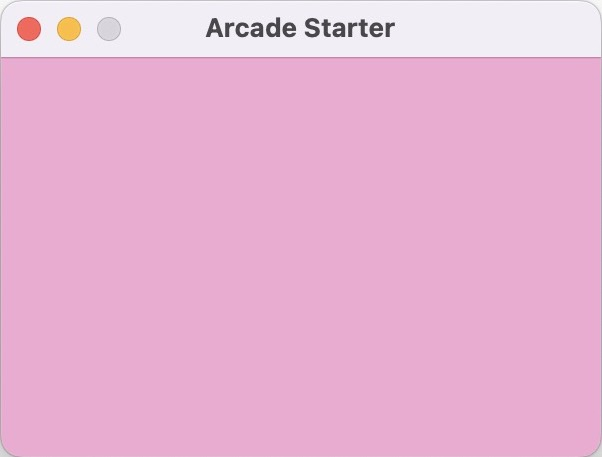
\includegraphics[width=.4\linewidth]{images/ch07/starter.jpg}};
    \drawshadow{image}
\end{tikzpicture}
\caption{}
\label{fig:ch07starter}
\end{figure}

အပေါ်ဆုံးမှာ \fCode{arcade} လိုက်ဘရီ အင်ပို့လုပ်ထားတာပါ။ ရှေ့ပိုင်းမှာသုံးတဲ့ \fCode{from} \fEnEmp{lib} \fCode{import *} ပုံစံ နဲ့ ကွာခြားတာက အခုနည်းနဲ့ အင်ပို့လုပ်ထားရင် လိုက်ဘရီမှာ ပါတဲ့ အစိတ်အပိုင်းတွေကို ဒေါ့ထ်အမှတ်အသားနဲ့ အသုံးပြုရပါမယ်။ ဥပမာ \fCode{open\_window} ဖန်ရှင်ကို
\begin{codetxt}
arcade.open_window(ß\fEnEmp{arguments}ß)
\end{codetxt} 
လိုက်ဘရီ နံမည်နောက်မှာ \fEn{(}\fCodeBf{.}\fEn{)} အမှတ်အသား ခံပြီး ခေါ်ရမှာပါ။ ဒီဖန်ရှင်မှာ လိုချင်တဲ့ဝင်းဒိုး အကျယ်၊ အမြင့်၊ တိုက်တယ်လ်စာသား ထည့်ပေးထားတယ်။ 

\fCode{set\_viewport} ဖန်ရှင်က ဝင်းဒိုးနေရာယူထားတဲ့ စခရင်ဧရီယာမှာ ကိုဩဒိနိတ်စစ်စတမ် သတ်မှတ်ပေးတာပါ။ \fEn{Origin} အမှတ်နဲ့  $x, y$ ဒါရိုက်ရှင် သတ်မှတ်ပေးတာပါ။
%
\begin{py}
arcade.set_viewport(left=0, right=300, top=0, bottom=200)
\end{py}
%
ဝင်းဒိုး ဘယ်ဘက်စွန်းကို $x = 0,$ ညာဘက်စွန်းကို $x = 300$ သတ်မှတ်ထားတယ်။ အပေါ်ဘက်စွန်း (တိုက်တယ်လ်ဘားမပါ) ကို $y = 0,$ အောက်ဘက်စွန်းကို $y = 200$ သတ်မှတ်ထားပါတယ်။ ဝင်းဒိုးရဲ့ ဘယ်ဘက်အပေါ်ထောင့်စွန်းက \fEn{origin} အမှတ် $(0,0)$ ဖြစ်တယ်။ ဘယ်ဘက်ကို သွားရင် $x$ တန်ဖိုး တိုးသွားပြီး အောက်ဘက်ကို ဆင်းရင် $y$ တန်ဖိုး တိုးသွားမှာဖြစ်တယ်။ အခုလို ကိုယ်တိုင်  မသတ်မှတ်ပေးဘဲ  သူ့နဂိုအရှိအတိုင်းဆိုရင် ‘အောက်ခြေ’ ဘယ်ဘက်စွန်းက \fEn{origin} ဖြစ်နေမှာပါ။ အောက်ခြေကနေ အပေါ်ကိုတက်သွားရင် $y$ တန်ဖိုး များလာမှာပါ။ သူ့နဂိုအတိုင်းက \fCode{set\_viewport} ကို အခုလိုခေါ်ထားတာဖြစ်မယ်။ \fCode{top=200}\fEn{,} \fCode{bottom=0} ပါ။
%
\begin{py}
arcade.set_viewport(left=0, right=300, top=200, bottom=0)
\end{py}
%
အသုံးများတဲ့ ဂိမ်းလိုက်ဘရီတွေမှာ ဒီစနစ်ကို သုံးကြတာ မတွေ့ရဘူး။ ဒီစနစ်နဲ့ အကျင့်ဖြစ်သွားရင် အခြားလိုက်ဘရီတွေ လေ့လာတဲ့အခါ အခက်အခဲရှိနိုင်တယ်။ အခုလေ့လာကြမဲ့ ဥပမာတွေ အတွက်လည်း အပေါ်မှာပြောတဲ့နည်းက ပိုအဆင်ပြေတယ်။ (\fEn{Arcade} ကိုပဲ တစိုက်မတ်မတ်သုံးမယ်၊ လေ့လာမယ်ဆိုရင်တော့ သူ့နဂိုအတိုင်းသုံးတာ အကောင်းဆုံးဖြစ်မှာပါ)။

အောက်ပါ ဖန်ရှင်ကတော့ ဝင်းဒိုးရဲ့ နောက်ခံရောင် သတ်မှတ်တာပါ။ လိုက်ဘရီရဲ့ \fCode{color} မော်ဒျူး \fEn{(\textit{module})} မှာ အရောင်တန်ဖိုးတွေ အဆင်သင့် သတ်မှတ်ပေးထားတယ်။ (မော်ဒျူးဆိုတာ လိုက်ဘရီရဲ့ အစိတ်အပိုင်းတစ်ခုလို့ အကြမ်းဖျဉ်း ယူဆနိုင်တယ်)။ 
%
\begin{py}
arcade.set_background_color(arcade.color.PINK_PEARL)
\end{py}
%
အခုလို အင်ပို့လုပ်ထားရင် အရောင်တွေ သုံးရတာ ပိုအဆင်ပြေတယ်
%
\begin{py}
import arcade
from arcade.color import *
ß$\ldots$ß
arcade.set_background_color(PINK_PEARL)
\end{py}
%
\fCode{PINK\_PEARL}\fEn{,} \fCode{RED} စသည်ဖြင့် အရောင်နံမည် တမ်းရေးလို့ရတယ်။ ရှေ့မှာ \fCode{arcade.color.} ထည့်ဖို့  မလိုတော့ဘူး။

ပုံဆွဲဖို့ အဆင်သင့်ဖြစ်အောင် \fCode{start\_render} ခေါ်ပေးရမယ်။ ဆွဲပြီးရင်လည်း \fCode{finish\_render} ခေါ်ဖို့လိုတယ်။ ပုံဆွဲတဲ့ကိစ္စကို ၎င်းတို့နှစ်ခုကြားမှာ  လုပ်ရမှာပါ။
%
\begin{py}
arcade.start_render()
# call drawing functions here
ß$\ldots$ß
ß$\ldots$ß
arcade.finish_render()
\end{py}
%
\betweenminted{\medskipamount}
%
\begin{py}
arcade.run()
\end{py}
%
ဝင်းဒိုးကို မပိတ်မချင်း ပေါ်နေအောင် \fCode{run} ဖန်ရှင် ခေါ်ပေးရတာပါ။ မခေါ်ထားဘဲ ပရိုဂရမ်ကို \fEn{run} ရင် ဝင်းဒိုးပွင့်လာပြီး ဖျတ်ခနဲ ပြန်ပိတ်သွားမှာပါ။ မကျန်ခဲ့ဖို့ သတိပြုရပါမယ်။

\fEn{Arcade} မှာ ပါတဲ့ အခြေခံ ပုံဆွဲဖန်ရှင် တချို့ကို ဆက်ကြည့်ရအောင်။ ထောင့်မှန်စတုဂံဆွဲတဲ့ ဖန်ရှင်တွေထဲက နှစ်ခု သုံးပြထားတယ်။ နှစ်ခုလုံးက  ထောင့်မှန်စတုဂံရဲ့ ဘယ်ဘက်အပေါ်ထောင့်စွန်းနဲ့ တည်နေရာကို သတ်မှတ်ပြီး အရွယ်အစားကို အကျယ်၊ အမြင့်နဲ့ သတ်မှတ်ပေးရတာပါ။  \fCode{draw\_xywh\_rec\allowbreak tangle\_filled} က အတွင်းပိုင်း အရောင်နဲ့ ဆွဲပေးတယ်။ အနားတွေကိုပဲ ဆွဲချင်ရင် \fCode{draw\_xywh\_rec\allowbreak tangle\_outline} ဖန်ရှင်သုံးရပါမယ်။
%
\begin{py}
import arcade
from arcade.color import *

arcade.open_window(300, 200, "Drawing Example")
arcade.set_viewport(0,300, 200, 0)

arcade.set_background_color(PINK_PEARL)
arcade.start_render()
# start drawing
arcade.draw_xywh_rectangle_filled(5,5,200, 50,BABY_BLUE)
arcade.draw_xywh_rectangle_outline(5,5,200, 50,BLACK)

arcade.draw_xywh_rectangle_filled(5,55,200, 50,PALE_VIOLET_RED)
arcade.draw_xywh_rectangle_outline(5,55,200, 50,BLACK)
#finish drawing
arcade.finish_render()
arcade.run()
\end{py}
%
အပေါ် ထောင့်မှန်စတုဂံပုံကို ဒီနှစ်ခုနဲ့ 
%
\begin{py}
arcade.draw_xywh_rectangle_filled(5,5,200, 50,BABY_BLUE)
arcade.draw_xywh_rectangle_outline(5,5,200, 50,BLACK)
\end{py}
%
ဆွဲထားတာပါ $\big\llbracket$ပုံ (\fRefNo{\ref{fig:ch07rects}})$\big\rrbracket$။ ပါရာမီတာတွေက $x, y, width, height, color$ အစဉ်အတိုင်းပဲ။ ဘယ်ဘက်ဘောင်ကနေ $x = 5$ ယူနစ် ခွာထားတယ်။  အပေါ်ဘောင်ကနေလည်း $y = 5$ ယူနစ်ခွာထားတယ်။ သုညထားပြီး စမ်းကြည့်ပါ။ အခြားတန်ဖိုးတွေ ထည့်ပြီး စမ်းကြည့်ပါ။ ပိုပြီးသဘောပေါက် လာပါလိမ့်မယ်။ ဒုတိယ ထောင့်မှန်စတုဂံက ဒီနှစ်ခုနဲ့
%
\begin{py}
arcade.draw_xywh_rectangle_filled(5,55,200, 50,PALE_VIOLET_RED)
arcade.draw_xywh_rectangle_outline(5,55,200, 50,BLACK)
\end{py}
%
ဆွဲထားတာပါ။ ဘယ်ဘက်ကို ခွာထားတာက အပေါ်ပုံနဲ့ တူတူပဲ $(x = 5)$။ အပေါ်ပုံရဲ့ အောက်ခြေအနားနဲ့ ကပ်နေအောင် $y = 5 + 50 (height) = 55$ ထားရပါမယ်။
\begin{figure}[tb!]
\begin{tikzpicture}
    \node[anchor=south west,inner sep=0] (image) at (0,0)
        {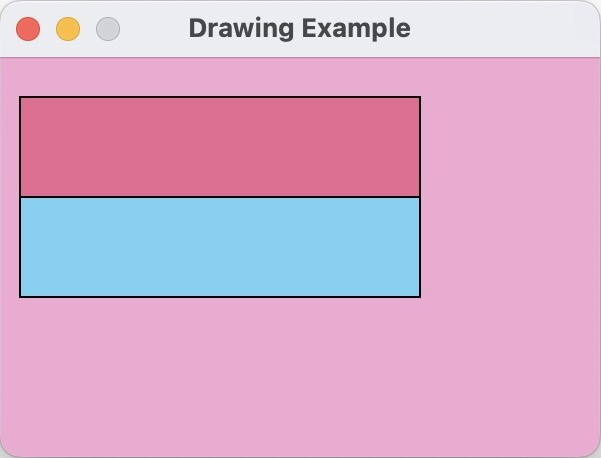
\includegraphics[width=.4\linewidth,trim={0mm 0mm 0mm 0.03mm}]{images/ch07/rects.jpg}};
    \drawshadow{image}
\end{tikzpicture}
\caption{}
\label{fig:ch07rects}
\end{figure}

\begin{mytcbox}
\qquad သူ့နဂိုအတိုင်းဆိုရင် \fEn{Arcade} ကိုဩဒိနိတ်စနစ်မှာ \fEn{origin} က  အောက်ခြေဘယ်ဘက်စွန်းလို့ ပြောခဲ့ပါတယ်။  \fCode{set\_viewport} နဲ့ အပေါ်ဘယ်ဘက်စွန်းကို \fEn{origin} အဖြစ်ပြောင်းလဲ သတ်မှတ်ထားတယ်။ ဒီ့အတွက်ကြောင့် အထက်အောက် ပြောင်းပြန်ဖြစ်သွားပါတယ်။ ဖန်ရှင် \fEn{documentation} မှာကြည့်ရင် အခုလိုတွေ့ရမှာပါ (\fEn{VS Code/PyCharm} မှာ  မောက်စ်ပွိုင်တာကို ဖန်ရှင်နံမည်ပေါ်မှာထားရင် \fEn{documentation} ပြပေးပါလိမ့်မယ်)
%
\begin{pytc}
def draw_xywh_rectangle_filled(bottom_left_x: float,
                               bottom_left_y: float,
                               width: float,
                               height: float,
                               color: tuple[int, int, int] 
                                   | list[int] 
                                   | tuple[int, int, int, int]) -> None
\end{pytc}
%
\fEn{Documentation} မှာ \fEn{bottom} ဆိုရင် ကိုယ့်အတွက် \fEn{top} လို့ ပြောင်းပြန် စဉ်းစားရမယ်။ သူ့နဂိုစနစ်ကို ပြောင်းလိုက်လို့ ဒီအခက်အခဲ ကြုံရတာပါ။ ဒါကြောင့် \fEn{Arcade} ကိုပဲ အဓိကသုံးမယ်ဆိုရင် သူ့အရှိအတိုင်းသုံးတာ အကောင်းဆုံးပဲ။ အထက်အောက် ပြောင်းပြန် စဉ်းစားစရာ မလိုတော့ဘူး။
\end{mytcbox}






\label{lst:checkerboard}
%
\begin{py}
import arcade
from arcade.color import *

WIN_WIDTH = 600
BOARD_SIZE = 400
WIN_HEIGHT = 420
arcade.open_window(WIN_WIDTH, WIN_HEIGHT, "Arcade Checkerboard")
arcade.set_viewport(left=0,
                    right=WIN_WIDTH,
                    top=0,
                    bottom=WIN_HEIGHT)
arcade.set_background_color(WHITE_SMOKE)
arcade.start_render()

COLS = 8
ROWS = 8
SQ_SIZE = BOARD_SIZE / ROWS
X_LFT = (WIN_WIDTH - BOARD_SIZE) / 2
Y_TOP = (WIN_HEIGHT - BOARD_SIZE) / 2 + 1

for i in range(ROWS):
    for j in range(COLS):
        x = X_LFT + SQ_SIZE * i
        y = Y_TOP + SQ_SIZE * j
        if (i + j) % 2 == 0:
            arcade.draw_xywh_rectangle_filled(x,
                                              y,
                                              SQ_SIZE,
                                              SQ_SIZE,
                                              WOOD_BROWN)
        else:
            arcade.draw_xywh_rectangle_filled(x,
                                              y,
                                              SQ_SIZE,
                                              SQ_SIZE,
                                              BLACK)
        arcade.draw_xywh_rectangle_outline(x,
                                           y,
                                           SQ_SIZE,
                                           SQ_SIZE,
                                           BLACK)

arcade.finish_render()
arcade.run()
\end{py}
%

\begin{figure}[tb!]
\begin{tikzpicture}
    \node[anchor=south west,inner sep=0] (image) at (0,0)
        {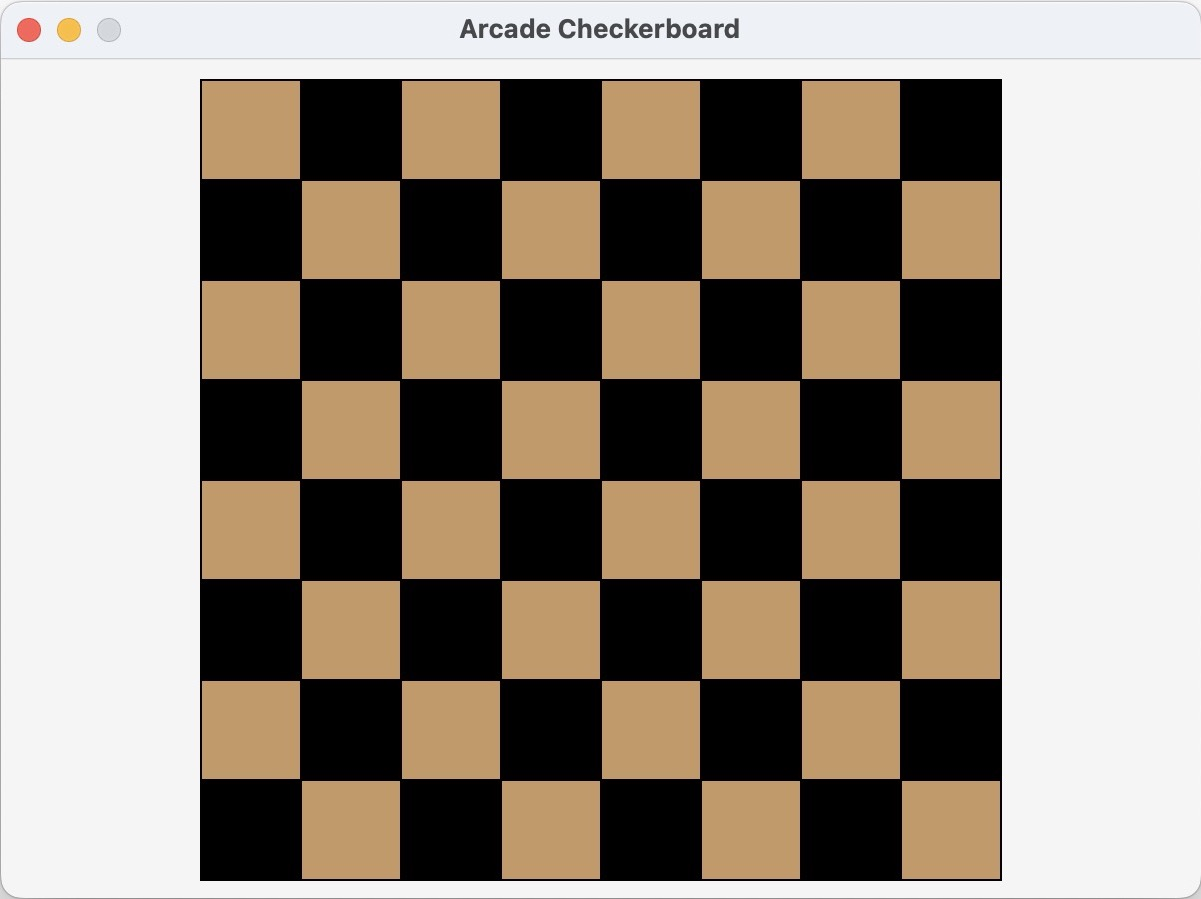
\includegraphics[width=.85\linewidth]{images/ch07/checkerboard.jpg}};
    \drawshadow{image}
\end{tikzpicture}
\caption{}
\label{fig:ch07chkbrd}
\end{figure}

\section{\fSecCodeBf{while} loop}
\fCode{while} \fEn{loop} ဟာ \fEnEmp{indefinite loop} ဖြစ်ပါတယ်။ \fEn{Loop} ကို စတင် လုပ်ဆောင်တဲ့အချိန်မှာ ဘယ်နှစ်ကြိမ် ပြန်ကျော့မလဲ အတိအကျ ကြို ‘မသိ’ ရင်  \fEn{indefinite loop} လို့ သတ်မှတ်တယ်။ တစ်နဲ့ တစ်ဆယ်ကြား (အပါအဝင်) ကိန်းပြည့်တစ်လုံးကို ကျပန်း \fEn{(random)} ထုတ်ထားမယ်။ မမှန်မချင်း အဲဒီဂဏန်းကို ခန့်မှန်းပေးရမယ်။ ခန့်မှန်းတာ မှန်သွားရင် ဘယ်နှစ်ခါ ခန့်မှန်းရလဲနဲ့ မှန်တဲ့ဂဏန်းကို ပြပေးတဲ့ ပရိုဂရမ်မှာ \fCode{while} \fEn{loop} အသုံးပြု ရေးထားတာ တွေ့ရပါမယ်။

%
\begin{py}
from random import *

num = randint(1, 10)

guess = int(input('? '))
times = 1
while guess != num:
    guess = int(input('? '))
    times += 1

print(f'You get correctly after {times} guesses.')
print(f'The number is {num}.')
\end{py}
%

\fCode{guess != num} (ဘူလီယန် အိပ်စ်ပရက်ရှင်) မမှားမချင်း \fEn{loop} က ပြန်ကျော့ပေးနေမှာပါ။ မှားတဲ့အခါ ထပ်မကျော့တော့ဘဲ ရပ်သွားမှာဖြစ်တယ်။ ကျပန်းဂဏန်းက ခုနှစ်ကျတယ် ဆိုပါစို့။ တစ်၊ ကိုး၊ သုံး၊ တစ်ဆယ်နဲ့ ခုနှစ် တို့ကို အစဉ်အတိုင်း ခန့်မှန်း ထည့်ပေးမယ်ဆိုရင် တစ်ကျော့ချင်း လိုက်ကြည့်တဲ့အခါ အခုလို တွေ့ရမှာပါ။

%
\begin{py}
num = randint(1, 10)            #ß 7 \fMM{ကျတယ် ယူဆပါ}ß

guess = int(input('? '))        #ß 1 \fMM{ထည့်ပေးတယ်}ß
times = 1

guess != num:                   #ß 1 != 7 \fMM{က \fCode{True}}ß
    ß\fEnBf{1\textsuperscript{\fEnBf{st}} iter:}ß
    guess = int(input('? '))    #ß 9 \fMM{ထည့်ပေးတယ် ယူဆပါ}ß
    times += 1                  #ß 2 \fMM{ဖြစ်သွားမယ်}ß

guess != num:                   #ß 9 != 7 \fMM{က \fCode{True}}ß
    ß\fEnBf{2\textsuperscript{\fEnBf{nd}} iter:}ß
    guess = int(input('? '))    #ß 3 \fMM{ထည့်ပေးတယ် ယူဆပါ}ß
    times += 1                  #ß 3 \fMM{ဖြစ်သွားမယ်}ß

guess != num:                   #ß 10 != 7 \fMM{က \fCode{True}}ß
    ß\fEnBf{3\textsuperscript{\fEnBf{rd}} iter:}ß
    guess = int(input('? '))    #ß 10 \fMM{ထည့်ပေးတယ် ယူဆပါ}ß
    times += 1                  #ß 4 \fMM{ဖြစ်သွားမယ်}ß

guess != num:                   #ß 7 != 7 \fMM{က \fCode{False} ဖြစ်သွားပြီ}ß
    #ß \fMM{ထပ်မကျော့တော့ဘူး}ß

#ß \fMM{\fEn{loop} အောက်က စတိတ်မန့်တွေ ဆက်လုပ်ပါတယ်}ß
print(f'You get correctly after {times} guesses.')
print(f'The number is {num}.')  
\end{py}
%

\fEn{Loop} က ထပ်မကျော့တော့ဘဲ  ရပ်သွားတာကို  \fEn{\textit{loop exits}} ဖြစ်သွားတယ်လို့ ပြောတယ်။ မြန်မာလိုတော့ \fEn{loop} ကနေ ထွက်သွားတယ်ပေါ့။ အကယ်၍ စောစောက ဥပမာမှာ ပထမဆုံးတစ်ခါမှာပဲ ခုနှစ် ထည့်လိုက်ရင်တော့ ဘလောက်ကို တစ်ခါမှ မလုပ်ဆောင်ဘဲ \fEn{loop} က ချက်ချင်းထွက်သွားမှာပါ။

\subsection*{Sentinel Controlled Loop}
ဂဏန်းတွေ ဘယ်နှစ်လုံး ပေါင်းမှာလဲ ကြိုသိရင် \fCode{for} \fEn{loop} နဲ့ အလုပ်ဖြစ်တယ်။ ဂဏန်း ဘယ်နှစ်လုံးရှိလဲ ကြိုမသိထားဘဲ ရှိသလောက် တစ်လုံးချင်းရိုက်ထည့်ပြီး အားလုံးပေါင်းချင်တာဆိုရင်တော့ \fCode{for} \fEn{loop} နဲ့ အဆင်မပြေဘူး (မရနိုင်ဘူးလို့ မဆိုလိုပါ၊ မရမက လုပ်တဲ့နည်းတွေလည်း ရှိပါတယ်)။ ဒီလိုအခြေအနေမျိုးမှာ \fEnEmp{sentinel controlled loop} ကို သုံးပါတယ်။ 

\fEn{Sentinel controlled loop} မှာ \fEn{loop} ကနေ ထွက်ဖို့အတွက် အသုံးပြုတဲ့ သီးသန့်တန်ဖိုးတစ်ခု ရှိရပါမယ်။ ဒီတန်ဖိုးကို \fEnEmp{sentinel value} လို့ ခေါ်တယ်။ ဂဏန်းတွေပေါင်းတဲ့ ကိစ္စအတွက်  \fEnEmp{sentinel value} ရွေးချယ်သတ်မှတ်တဲ့အခါ ပေါင်းရမဲ့ဂဏန်း မဖြစ်နိုင်တဲ့ တစ်ခုကို ရွေးရပါမယ်။ သုညဟာ အပေါင်းထပ်တူရ ဂုဏ်သတ္တိရှိတဲ့အတွက် ၎င်းကို \fEnEmp{sentinel value} အဖြစ် ထားနိုင်တယ်။
%
\begin{py}
# File: add_nums_sentinel.py 
SENTINEL = 0
total = 0

val = int(input('? '))
while val != SENTINEL:
    total += val
    val = int(input('? '))

print(f'Total is {total}')
\end{py}
%
ထည့်ပေးတဲ့ ဂဏန်းဟာ သုညမဟုတ်မချင်း \fCode{total} မှာ ပေါင်းထည့်ပြီး နောက်ဂဏန်းတစ်ခု ထည့်ပေးဖို့ \fEn{input} တောင်းမှာပါ။ \fEn{Sentinel} တန်ဖိုး သုည ထည့်လိုက်ရင် \fEn{loop} က ထွက်သွားမယ်။ ပြီးတဲ့အခါ \fCode{total} ကို ပြပေးမှာပါ။ စစချင်းပဲ သုည ထည့်လိုက်ရင် \fEn{loop} က တစ်ခါမှ မကျော့ဘဲ ထွက်သွားမယ်။ \fCode{total} လည်း သုညပဲ ထွက်ပါမယ်။ အခုပရိုဂရမ်ကို နောက်တစ်နည်း ရေးလို့ရပါတယ်။ 
%
\begin{py}
# File: add_nums_sentinel2.py 
SENTINEL = 0
total = 0

while True:
    val = int(input('? '))
    if val == SENTINEL:
        break
    total += val

print(f'Total is {total}')

\end{py}
%

\fCode{while True:} က ပုံမှန်ဆိုရင် \fEn{infinite loop} ဖြစ်ပါလိမ့်မယ်။ အမြဲမှန်နေတဲ့အတွက် ပြန်ကျော့တာ ဘယ်တော့မှ ရပ်မှာ မဟုတ်ဘူး။ ဒီလိုဖြစ်နေတာကို ဖြတ်ချပစ်ဖို့အတွက် \fCode{break} စတိတ်မန့်ကို သုံးထားပါတယ်။ \fCode{if val == SENTINEL:} (ထည့်ပေးတဲ့ တန်ဖိုးက သုညဆိုရင်) လက်ရှိ အလုပ်လုပ်နေတဲ့ \fEn{loop} ကို \fCode{break} လိုက်မှာဖြစ်တယ်။ 

အထက်ပါ \fEn{sentinel loop} ပုံစံနှစ်ခုကို ယှဉ်ကြည့်ရင်  ပထမတစ်ခုမှာ \fEn{input} တန်ဖိုးထည့်ခိုင်းတာကို \fEn{loop} မစမီ တစ်ခါ ကြိုလုပ်ထားရတယ်။ နောက်တစ်ခုမှာတော့ အဲ့ဒီလို ကြိုလုပ်ထားစရာမလိုဘူး။ \fEn{Loop} ဘလောက်ထဲက စတိတ်မန့်တစ်ခုကို အပြင်မှာထုတ်ထားရတဲ့အတွက် တချို့က ပထမပုံစံထက် ဒုတိယပုံစံက ကုဒ်စတိုင်လ်အားဖြင့် ပိုပြီး သပ်ရပ်ကြော့ရှင်းတယ်လို့ ယူဆကြပါတယ်။

\subsection*{Result Controlled Loop}

တစ်နှစ်ငါးရာခိုင်နှုန်း အတိုးနဲ့ ဘဏ်မှာ ဒေါ်လာတစ်ထောင် စုထားတယ်။ တစ်နှစ်ပြည့်တိုင်း အတိုးအရင်း ပေါင်းပြီး နောက်နှစ်အတွက် အတိုးတွက်တယ်။ နှစ်ထပ်တိုး \fEn{(yearly compound interest)} လို့ခေါ်ပါတယ်။ ဒီနည်းလမ်းနဲ့ အနည်းဆုံး ဒေါ်လာတစ်သန်း စုမိဖို့ (မီလျံနာတစ်ယောက်ဖြစ်ဖို့) ဘယ်နှစ်နှစ်စောင့်ရမလဲ။ သုံးနှစ်ပြည့်ရင် စုမိမဲ့ ငွေပမာဏ တွက်ထားတာကို ကြည့်ပါ။


%
\begin{flushleft}
\vspace{1em}
\setlength{\extrarowheight}{3pt}
\begin{tabular}[h]{*{3}l l l}
    \toprule[1.5pt]
        \fTblHead{Year} & \fTblHead{Interest} & \fTblHead{Balance}\\       
    \midrule
    $1$ & $1000 \times 0.05 = 50$ & $1000 + 50 = 1050$\\
    $2$ & $1050 \times 0.05 = 52.5$ & $1050 + 52.5 = 1102.5$\\
    $3$ & $1102.5 \times 0.05 = 55.125$ & $1102.5 + 55.125 = 1157.625$\\   
    \bottomrule[1.5pt]
\end{tabular}
\label{tbl:ch07onem}
\captionof{table}{သုံးနှစ်စာ နှစ်ထပ်တိုး}
\end{flushleft}
%

ဒေါ်လာတစ်သန်း အနည်းဆုံးရဖို့ နှစ်ဘယ်လောက်ကြာမလဲ အခုလို ရှာနိုင်ပါတယ် 


% https://realpython.com/python-f-strings/
%
\begin{py}
# File: one_million.py
balance = 1000
INT_RATE = 0.05
TARGET = 1_000_000
yr = 0

print(f"{'yr':>4s} {'interest':>10s} {'balance':>10s}")
while balance < TARGET:
    interest = balance * INT_RATE
    balance += interest
    yr += 1
    print(f'{yr:4d} {interest:10.2f} {balance:10.2f}')

print(f'You have to wait {yr} years!')
\end{py}
%
\fCode{while} \fEn{loop} ထဲမှာ တစ်နှစ်ကုန်တဲ့အခါ ရမဲ့ အတိုးနဲ့ အတိုးအရင်းပေါင်း တွက်ထားပြီး  \fCode{yr} ကိုလည်း တစ်နှစ် တိုးပေးတယ်။ \fCode{yr}\fEn{,} \fCode{interest}\fEn{,} \fCode{balance} ထုတ်ပြပေးတယ် (မပြလည်း ပြဿနာမရှိပါ၊ တစ်နှစ်စာ တွက်ထားတာ စစ်ကြည့်လို့ရအောင် ထုတ်ကြည့်တာပါ)။ တစ်သန်းမပြည့်မချင်း ပြန်ကျော့ပေးအောင် \fEn{loop} ကွန်ဒီရှင်ကို \fCode{balance < TARGET} နဲ့ စစ်ထားတယ်။ တစ်သန်းနဲ့ညီရင် (သို့) တစ်သန်းကျော်သွားတာနဲ့ ကွန်ဒီရှင် \fCode{False} ဖြစ်သွားပြီး ထပ်မကျော့တော့ဘူး။ \fEn{Loop} တစ်ခါကျော့တိုင်း တစ်နှစ်စာ အတိုးအရင်းပေါင်း \fCode{balance} ကို တွက်ချက်ပြီး \fEn{loop} ကနေ ဘယ်အချိန် ထွက်မလဲကလည်း အဲဒီရလဒ်အပေါ် မူတည်နေတာ တွေ့ရပါမယ်။ ဒီလို သဘောတရားရှိတဲ့ \fEn{loop} မျိုးကို \fEn{result controlled loop} လို့ ခေါ်ပါတယ်။ ကျော့မဲ့ အကြိမ်အရေအတွက်က \fEn{loop} ထဲမှာ တွက်ချက်ထားတဲ့ ရလဒ်ပေါ် မူတည်တယ်။

ပရိုဂရမ် \fEn{output} ကို အခုလို ကော်လံတစ်ခုစီကို အကျယ် တစ်သမတ်တည်းဖြစ်၊ စာသားတွေ ညာဘက်ကပ်ပြီး ညီနေအောင် \fEn{f-strings} ကို \fEn{format spec} လို့ခေါ်တဲ့ ဖော့မတ်သတ်မှတ်တဲ့ နည်းစနစ်ကို သုံးထားတာပါ။
\begin{codetxt}
  yr   interest    balance
   1      50.00    1050.00
   2      52.50    1102.50
 ...      ...      ...    
 142   48602.79 1020658.53
You have to wait 142 years!
\end{codetxt}
\fEn{Format spec} နဲ့ ပါတ်သက်ပြီး အကျယ်တဝင့် မဖော်ပြတော့ဘဲ အခုလို ဖော့မတ်ရအောင် ဘယ်လိုလုပ်ထားလဲကိုပဲ ရှင်းပြပါမယ်။
%
\begin{py}
f"{'yr':>4s} {'interest':>10s} {'balance':>10s}"
\end{py}
%
ကော်လံ ခေါင်းစည်း အတွက် \fEn{f-string} ပါ။ ဖော့မတ်လုပ်ရမဲ့ တန်ဖိုး/ဗေရီရေဘဲလ်/အိပ်စ်ပရက်ရှင်က \fCode{:} (ကော်လံ) ဘယ်ဘက်မှာ ရှိမယ်။ ညာဘက်မှာ  \fEn{format spec} ရှိမယ်။ \fCodeBf{>4s} က \fCode{'yr'} အတွက် \fEn{format spec} ဖြစ်တယ်။ \fCodeBf{>} က ညာဘက်ကပ်ဖို့၊ \fCodeBf{4} က ကော်လံအကျယ်ကို ကာရက်တာ လေးလုံးသတ်မှတ်တာ။ \fCodeBf{s} ကတော့ တန်ဖိုးကို \fEn{string} အနေနဲ့ ပြပေးပါလို ဆိုလိုတယ်။ ကျန်တဲ့ ကော်လံနှစ်ခု အတွက် \fEn{format spec} ကို \fCodeBf{>10s} သတ်မှတ်တယ်။  ကာရက်တာ ဆယ်လုံး ကော်လံအကျယ် သတ်မှတ်တယ်။
%
\begin{py}
f'{yr:4d} {interest:10.2f} {balance:10.2f}'
\end{py}
%
ဒါကတော့ \fCode{yr}\fEn{,} \fCode{interest}\fEn{,} \fCode{balance} တန်ဖိုးတွေကို ပြပေးဖို့ပါ။ ကော်လံအကျယ် \fCode{4}\fEn{,} \fCode{10}\fEn{,} \fCode{10} သတ်မှတ်တယ်။ \fCode{yr} ကို ကိန်းပြည်ဂဏန်းအနေနဲ့ ပြပေးအောင် \fCode{d} သုံးတယ်။ ကျန်တဲ့နှစ်ခုကို ဒဿမနဲ့ ပြဖို့ \fCode{f} သုံးတယ်။ \fCode{.2} ကတော့ ဒဿမနောက် ဂဏန်းနှစ်လုံး ပြပေးခိုင်းတာ။ ကိန်းဂဏန်းဆိုရင် သူ့နဂိုအတိုင်း ညာဘက်ကပ်ပေးတဲ့အတွက် \fCode{>} ထည့်ဖို့ မလိုဘူး။ ဘယ်ဘက်ကပ်ချင်ရင် \fCode{<} သုံးလို့ရတယ်။

\section{လေ့ကျင့်ရန် ဥပမာများ}

ကွန်ထရိုးလ် စထရက်ချာတွေ အသုံးချတတ်လာအောင် များများလေ့ကျင့်၊ များများစဉ်းစား၊ များများရေးကြည့် ရမှာပါ။ ဘယ်အတတ်ပညာမဆို များများလေ့ကျင့်မှ ကျွမ်းကျင်လာနိုင်မှာပါ။ ဒီသဘောအရ ပရိုဂရမ်းမင်း ပညာရပ်ဟာလည်း ချွင်းချက်မဖြစ်နိုင်ပါဘူး။

\begin{mytcbox}
အောက်ပါ ဥပမာတစ်ခုချင်းကို ပုစ္ဆာနားလည်အောင်ဖတ်ပြီး ကိုယ်တိုင်စဉ်းစား ရေးကြည့်ဖို့ လေးလေးနက်နက် အကြံပြုပါတယ်။ ရေးပြီးသွားရင် ပုစ္ဆာမှာ ဖော်ပြထားချက်နဲ့ အညီ အလုပ်လုပ်/မလုပ် ဟာကွက်မရှိအောင် ဘယ်လိုစစ်ဆေး စိစစ်မလဲ မိမိဘာသာ စဉ်းစားကြည့်ပါ။
\end{mytcbox}

\subsection*{Internet Delicatessen}
\fEn{Online} ကနေ အစားအသောက်တွေ \fEn{delivery} ပို့ပေးဖို့ အမှာလက်ခံတဲ့ ဆိုင်လေးတစ်ဆိုင်အတွက် ပရိုဂရမ်ရေးပေးရပါမယ်။ အော်ဒါမှာတဲ့အခါ မှာမဲ့ အစားအသောက် နံမည်၊ ဈေးနှုန်းနဲ့ အိပ်စ်ပရက်စ် \fEn{delivery} ယူမယူ ပရိုဂရမ်မှာ ထည့်ပေးရပါမယ်။ ပရိုဂရမ်က အော်ဒါနဲ့ စုစုပေါင်းကျသင့်ငွေကို ထုတ်ပေးရပါမယ်။ တစ်သောင်းနဲ့အထက်မှာရင် \fEn{delivery} ဖိုး ပေးစရာမလိုပါ။ တစ်သောင်းအောက်ဆိုရင်တော့ နှစ်ရာပေးရပါမယ်။ အိပ်စ်ပရက်စ် \fEn{delivery} ယူမယ်ဆိုရင် သုံးရာအပို ထပ်ပေးရပါမယ်။
%
\begin{minted}[frame=lines, framerule=0pt,escapeinside=ßß]{text}
ß\fEn{Enter the item: Tuna Salad}ß
ß\fEn{Enter the price: 4500}ß
ß\fEn{Express delivery (0==no, 1==yes): 1}ß

ß\fEn{Invoice:}ß
ß\fEn{Tuna Salad\space\space 4500}ß
ß\fEn{delivery\space\space\space\space\space\space\space 500}ß 
ß\fEn{total\space\space\space\space\space\space\space\space\space\space\space 5000}ß
\end{minted}
%

%
\begin{py}
itm_name = input('Item name: ')
price = int(input('Price: '))
is_exp_deli = int(input('Express delivery (0==no, 1==yes): '))

tot_deli_fee = 0
if price >= 10_000 and is_exp_deli == 1:
    tot_deli_fee = 300
elif price >= 10_000 and is_exp_deli == 0:
    tot_deli_fee = 0
elif price < 10_000 and is_exp_deli == 1:
    tot_deli_fee = 200 + 300
elif price < 10_000 and is_exp_deli == 0:
    tot_deli_fee = 200
else:
    print("You may have wrong value for express deli.")

tot_cost = price + tot_deli_fee

print("Invoice: ")
print(f'{itm_name:<10s} {price:8.2f}')
print(f"{'delivery':<10s} {tot_deli_fee:8.2f}")
print(f"{'total':<10s} {tot_cost:8.2f}")
\end{py}
အိပ်စ်ပရက်စ် \fEn{delivery} ယူ/မယူ တစ် (သို့) သုည ထည့်ပေးရမှာပါ။ တစ်/သုည မဟုတ်တဲ့ ဂဏန်းတစ်ခု မှားထည့်မိရင် \fCode{if...elif} ကွန်ဒီရှင်တွေ တစ်ခုမှ \fCode{True} ဖြစ်မှာ မဟုတ်ပါဘူး။ မှားထည့်ထားတယ်လို့ သတိပေးဖို့ \fCode{else} အပိုင်းမှာ လုပ်ထားတယ်။ မှန်/မမှန် စိစစ်တဲ့အခါ အောက်ပါဇယားမှ ဖြစ်နိုင်ခြေအားလုံး ခြုံငုံမိအောင် စစ်သင့်တယ်။ အိပ်စ်ပရက်စ် \fEn{delivery} အတွက် \fEn{input} ဂဏန်း မှားထည့်ရင် သတိပေးတာကိုလည်း စစ်သင့်တယ်။ တစ်သောင်းဖိုး ဝယ်တာကို သုံးမျိုးစစ်ထားတာ လေ့လာကြည့်ပါ။ တစ်သောင်း မပြည့်တာနဲ့ တစ်သောင်းကျော်ဖိုး အတွက်လည်း အလားတူ စစ်ကြည့်လို့ အားလုံးမှန်တယ်ဆိုရင် ဒီပရိုဂရမ်မှာ \fEn{bug} ပါနိုင်ခြေ လုံးဝမရှိသလာက် ဖြစ်သွားပါပြီ။ 

%
\begin{flushleft}
\vspace{1em}
\setlength{\extrarowheight}{3pt}
\begin{tabular}[h]{*{3}l l l}
    \toprule[1.5pt]
        \fTblHead{10,000 MMK and above?} & \fTblHead{Express Delivery?}\\       
    \midrule
    \fEn{Yes} & \fEn{Yes}  \\
    \fEn{Yes} & \fEn{No}   \\
    \fEn{No}  & \fEn{Yes}  \\
    \fEn{No}  & \fEn{No}   \\
       
    \bottomrule[1.5pt]
\end{tabular}
\label{tbl:ch07inetdeli}
\captionof{table}{သုံးနှစ်စာ နှစ်ထပ်တိုး}
\end{flushleft}
%
\vspace*{1em}
\noindent\fEn{Test Output:}
\begin{codetxt}
Item name: Salad
Price: 10000
Express delivery (0==no, 1==yes): 1
Invoice: 
Salad      10000.00
delivery     300.00
total      10300.00
\end{codetxt}
\betweenminted{\medskipamount}
\begin{codetxt}
Item name: Salad
Price: 10000
Express delivery (0==no, 1==yes): 0
Invoice: 
Salad      10000.00
delivery       0.00
total      10000.00
\end{codetxt}
\betweenminted{\medskipamount}
\begin{codetxt}
Item name: Salad
Price: 10000
Express delivery (0==no, 1==yes): 2
You may have wrong value for express deli.
Invoice: 
Salad      10000.00
delivery       0.00
total      10000.00
\end{codetxt}

ပရိုဂရမ်တစ်ခုရဲ့ လိုအပ်ချက်ဟာ မကြာခဏ ပြောင်းလဲသွားလေ့ရှိတယ်။ အခုပရိုဂရမ်မှာ ဈေးနှုန်းသတ်မှတ်ချက်တွေ ပြောင်းလဲနိုင်တယ်။ အနည်းဆုံး တစ်သောင်းခွဲဝယ်မှ ပို့ခ \fEn{free} ရမှာဖြစ်ပြီး တစ်သောင်းခွဲအောက်ဆိုရင် ပို့ခ သုံးရာ့ငါးဆယ် ပြောင်းလဲသတ်မှတ်လိုက်တဲ့အပြင် အိပ်စ်ပရက်စ် \fEn{delivery} ကလည်း တစ်ရာဈေးထပ်တက်သွားတယ် ဆိုပါစို့။ တကယ့်လက်တွေ့မှာလည်း ဒါမျိုးဖြစ်လေ့ရှိပါတယ်။ ဒီအတွက်ကို ပရိုဂရမ်ကို ပြင်ပေးရပါမယ်။ ဆိုင်ပိုင်ရှင်ကလည်း ဈေးနှုန်းမကြာခဏ ပြောင်းဖို့လိုနိုင်ကြောင်း ပြောလာပါတယ်။ နောင်လည်း ထပ်ပြင်ပေးဖို့လိုမဲ့ သဘောပါ။ လွယ်လွယ်ကူကူ ပြင်ပေးနိုင်ရင် အကောင်းဆုံးပါ။ ပြင်ဆင်တဲ့အခါ မှားနိုင်ခြေနည်းဖို့လည်း အရေးကြီးပါတယ်။ ခုရေးထားတဲ့အတိုင်းဆိုရင် ပြီးခဲ့တဲ့ပရိုဂရမ်မှာ ပြဿနာရှိနေပါတယ်။

ပြီးခဲ့တဲ့ ပရိုဂရမ်မှာ ပြင်မယ်ဆိုရင် \fCode{10\_000} ကို လေးနေရာ၊ ပုံမှန်ပို့ခ \fCode{200} နဲ့ အိပ်စ်ပရက်စ်အပိုကြေး \fCode{300} စတာတွေကို နှစ်နေရာစီ လိုက်ပြင်ရပါမယ်။ အလုပ်ရှုပ်တဲ့အပြင် ပြင်ဖို့ကျန်ခဲ့တာလို့  မှားတာလည်း ဖြစ်နိုင်တယ်။ \fEn{“Find and Replace”} လုပ်မှာပေါ့လို့ စောဒကတက်စရာ ရှိပါတယ်။ အခုလို ကုဒ်လိုင်း နည်းနည်းပဲရှိတဲ့ ပရိုဂရမ်အသေးလေးမှာ အဆင်ပြေနိုင်ပေမဲ့ ပိုရှုပ်ထွေးပြီး ကုဒ်လိုင်းတွေများတဲ့ ပရိုဂရမ်မျိုးတွေမှာ \fEn{“Find and Replace”} လုပ်ရင် မပြင်သင့်တာတွေကိုပါ မရည်ရွယ်ပဲ ပြင်မိသွားတာဖြစ်တတ်ပါတယ်။ ပရိုဂရမ်ရေးတဲ့အခါ ကျင့်သုံးရမဲ့ အလေ့အထကောင်းတစ်ခုက ကုဒ်ထဲမှာ ဒီတိုင်းချရေးထားတဲ့ တန်ဖိုးတွေ \fEn{(literal constants)} တွေကို နာမည်ပေးထားတာပါ။ အပေါ်က ပရိုဂရမ်မှာ \fEn{literal constants} တွေချည်း သုံးထားတယ်။ နံမည်ပေးထားတဲ့ \fEn{constants} \fEn{(named constants)} တွေအဖြစ် ပြောင်းရေးသင့်တယ်။
%
\begin{py}
FREE_DELI_AMT = 15_000
DELI_FEE = 350
EXP_DELI_FEE = 400

itm_name = input('Item name: ')
price = int(input('Price: '))
is_exp_deli = int(input('Express delivery (0==no, 1==yes): '))

tot_deli_fee = 0

if price >= FREE_DELI_AMT and is_exp_deli == 1:
    tot_deli_fee = EXP_DELI_FEE
elif price >= FREE_DELI_AMT and is_exp_deli == 0:
    tot_deli_fee = 0
elif price < FREE_DELI_AMT and is_exp_deli == 1:
    tot_deli_fee = DELI_FEE + EXP_DELI_FEE
elif price < FREE_DELI_AMT and is_exp_deli == 0:
    tot_deli_fee = DELI_FEE
else:
    print("You may have wrong value for express deli.")

tot_cost = price + tot_deli_fee
print("Invoice: ")
print(f'%-10s %8.2f' % (itm_name, price))
print(f'%-10s %8.2f' % ('delivery', tot_deli_fee))
print(f'%-10s %8.2f' % ('total', tot_cost))
\end{py}
%

ဒီပရိုဂရမ်ကို \fEn{cascading} \fCode{if} မသုံးဘဲ ရိုးရိုး \fCode{if} နဲ့ ရေးလို့လည်း ရတယ်။ 
%
\begin{py}
FREE_DELI_AMT = 15_000
DELI_FEE = 350
EXP_DELI_FEE = 400

itm_name = input('Item name: ')
price = int(input('Price: '))
is_exp_deli = int(input('Express delivery (0==no, 1==yes): '))

tot_deli_fee = 0

if price < FREE_DELI_AMT:
    tot_deli_fee += DELI_FEE

if is_exp_deli == 1:
    tot_deli_fee += EXP_DELI_FEE

if not (is_exp_deli == 0 or is_exp_deli == 1):
    print("You may have wrong value for express deli.")

tot_cost = price + tot_deli_fee

print("Invoice: ")
print(f'%-10s %8.2f' % (itm_name, price))
print(f'%-10s %8.2f' % ('delivery', tot_deli_fee))
print(f'%-10s %8.2f' % ('total', tot_cost))
\end{py}
%
ပထမ \fCode{if} က \fEn{delivery} ခ ပေးဖို့ လိုတယ်ဆိုရင် \fCode{tot\_deli\_fee} မှာ \fCode{DELI\_FEE} ပေါင်းထည့်ပေးတယ်။ ဒုတိယ \fCode{if} က အိပ်စ်ပရက်စ် \fEn{delivery} ယူမယ်ဆိုရင် \fCode{tot\_deli\_fee} မှာ \fCode{EXP\_DELI\_FEE} ထပ်ပေါင်းထည့်တယ်။ အောက်ဆုံး \fCode{if} ကတော့ အိပ်စ်ပရက်စ် \fEn{delivery} အတွက် တစ်နဲ့ သုည မဟုတ်တာ ထည့်မိရင် သတိပေးစာသား ပြပေးတယ်။

ဒီပရိုဂရမ်နဲ့ ဒီ့မတိုင်ခင် သူ့ရှေ့က ပရိုဂရမ်က ဖြစ်နိုင်ခြေအားလုံးအတွက်တော့ ရလဒ် တူတူမထွက်ပါဘူး။  အခြေအနေ တစ်ခုကလွဲလို့ ကျန်တာတွေအတွက်တော့ ရလဒ်တူပါတယ်။ တစ်သောင်းငါးထောင် ထက်ငယ်တဲ့ တန်ဖိုးနဲ့ အိပ်စ်ပရက်စ် \fEn{delivery} အတွက် ဂဏန်း လွဲထည့်ကြည့်ပါ။ ဥပမာ

\begin{codetxt}
Item name: salad
Price: 12000
Express delivery (0==no, 1==yes): 2
You may have wrong value for express deli.
Invoice: 
salad      12000.00
delivery       0.00
total      12000.00
\end{codetxt}
\betweenminted{\medskipamount}
\begin{codetxt}
Item name: salad
Price: 12000
Express delivery (0==no, 1==yes): 2
You may have wrong value for express deli.
Invoice: 
salad      12000.00
delivery     ß\textbf{350.00}ß
total      ß\textbf{12350.00}ß
\end{codetxt}
နောက်ဆုံး ပရိုဂရမ်က အိပ်စ်ပရက်စ် \fEn{delivery} အတွက် မပေါင်းထည့်ပေမဲ့ ပုံမှန် \fEn{delivery} ခ သုံးရာ့ငါးဆယ်ကိုတော့ ထည့်ပေါင်းသွားတာ တွေ့ရမယ်။ မှားထည့်တာကိုပဲ သတိပေးစာသားပြပေးတာ၊ ထည့်မတွက်သွားတာက ပိုပြီး သဘာဝကျတယ်လို့ ယူဆရမှာပါ။

\begin{mytcbox}
ပြင်ပကနေ ထည့်ပေးတဲ့အခါ မဖြစ်သင့်တဲ့ \fEn{input} တန်ဖိုးတွေ ဝင်မလာအောင် စိစစ်တာကို \fEn{input validation} လို့ ခေါ်တယ်။ တကယ့် လက်တွေ့ အသုံးချ ပရိုဂရမ်တွေမှာ \fEn{input validation} လုပ်ထားဖို့ အရေးကြီးပေမဲ့ ဘီဂင်နာအဆင့် လေ့လာတဲ့ ဥပမာတွေမှာတော့ လေ့လာရင်းကိစ္စကနေ လမ်းကြောင်းမချော်သွားအောင် ဆင်ခြင်ရမှာဖြစ်ပြီး သင့်တော်ရုံ ဆက်စပ်ရှင်းပြပါမယ်။ 
\end{mytcbox}

\subsection*{တာရာ ပရက်ရှာ}

ကားဘီးလေထိုးတာဟာ ကားရဲ့ စွမ်းဆောင်ရည်ရော အန္တရာယ်ကင်းဖို့အတွက်ပါ ပဓာနကျပါတယ်။ ကားတစ်စီးအတွက် အကြံပြုထားတဲ့ တာယာပရက်ရှာ \fEn{(recommended pressure)} အပေါ် မူတည်ပြီး လေဘယ်လောက်တင်းလို့ရလဲ၊ လျော့လို့ရလဲ ရှိပါတယ်။ ဥပမာ \fEn{recommended pressure} က \fEn{35 psi (pounds per square inch)} ဖြစ်ရင် အလွန်ဆုံး \fEn{31.5 psi} ထိ လေလျော့လို့ရပါတယ်။ လေပိုတင်းမယ်ဆိုရင်လည်း အလွန့်အလွန်ဆုံး \fEn{44 psi} အထိ ရပါနိုင်ပါတယ်။

ရှေ့တာယာနှစ်လုံး ပရက်ရှာအနီးစပ်ဆုံးတူသင့်ပြီး \fEn{3 psi} အထိ ကွာဟလို့ရတယ်။ ကွာဟချက်က \fEn{3 psi} ထက်တော့ မများသင့်ဘူး။ နောက်တာယာနှစ်လုံးလည်း ထိုနည်းတူစွာပဲ ဖြစ်တယ်။ ကားမော်ဒယ်အလိုက် \fEn{recommended pressure} ကွာခြားပေမဲ့ အိမ်စီးကားအများစုအတွက် \fEn{35 psi} ဖြစ်တယ်လို့ယူဆပြီး တာယာပရက်ရှာ အိုကေမကေ စစ်ပေးတဲ့ ပရိုဂရမ် ရေးပေးရပါမယ်။ \fEn{Input} အနေနဲ့ တာယာတစ်ခုချင်းအတွက် ပရက်ရှာ \fEn{psi} တန်ဖိုး ထည့်ပေးရမှာပါ။ ထည့်ပေးလိုက်တဲ့ တာယာပရက်ရှာ \fEn{31.5 psi} ထက်နည်းနေရင် သို့မဟုတ် \fEn{44 psi} ထက်များနေတာနဲ့ သတ်မှတ်ဘောင် မဝင် \fEn{(out of range)} ဖြစ်နေကြောင်း သတိပေးရပါမယ်။ တာယာအားလုံးရဲ့ ပရက်ရှာတွေ သတ်မှတ်ဘောင်အတွင်း ဝင်တယ်၊ ရှေ့တာယာနှစ်လုံး ကွာဟချက်၊ နောက်တာယာနှစ်လုံး ကွာဟချက်တွေ ခွင့်ပြုလို့ရတာထက် မပိုဘူးဆိုရင် လေထိုးထားတာ အိုကေတယ်။ တာယာတစ်လုံး \fEn{out of range} ဖြစ်နေတာနဲ့ လေထိုးထားတာ မအိုကေဘူး ပြပေးရပါမယ်။

% https://blog.nationwide.com/vehicle/vehicle-maintenance/recommended-tire-pressure/
%
%
\begin{py}
MIN_ALLOWABLE = 31.5
MAX_ALLOWABLE = 44.0
WARNING = 'Waring: Pressure is out of range!'
LEFT_RIGHT_DIFF_ALLOWABLE = 3.0

is_out_of_range = False

front_left = float(input("Front left pressure: "))
if not (MIN_ALLOWABLE <= front_left <= MAX_ALLOWABLE):
    is_out_of_range = True
    print(WARNING)

front_right = float(input("Front right pressure: "))
if not (MIN_ALLOWABLE <= front_right <= MAX_ALLOWABLE):
    is_out_of_range = True
    print(WARNING)

rear_left = float(input("Rear left pressure: "))
if not (MIN_ALLOWABLE <= rear_left <= MAX_ALLOWABLE):
    is_out_of_range = True
    print(WARNING)

rear_right = float(input("Rear right pressure: "))
if not (MIN_ALLOWABLE <= rear_right <= MAX_ALLOWABLE):
    is_out_of_range = True
    print(WARNING)

front_diff = abs(front_left - front_right)
front_diff = abs(rear_left - rear_right)
if (front_diff <= LEFT_RIGHT_DIFF_ALLOWABLE
        and rear_diff <= LEFT_RIGHT_DIFF_ALLOWABLE
        and not is_out_of_range):
    print("Inflation is OK.")
else:
    print("Inflation is not OK!")

\end{py}
%

\fCode{is\_out\_of\_range} ဘူလီယန် သုံးထားတာ နည်းနည်း ရှင်းပြဖို့ လိုပါမယ်။ စစချင်း \fCode{False} တန်ဖိုး ထည့်ထားတာ တွေ့ရမှာပါ။ \fCode{if} စတိတ်မန့်တွေက တာယာတစ်ခုချင်းကို \fEn{out of range} ဖြစ်နေလား စစ်ထားတာတွေ့ရတယ်။ တာယာတစ်ခု \fEn{out of range} ဖြစ်တာနဲ့ \fCode{is\_out\_of\_range} က \fCode{True} ဖြစ်သွားမှာပါ။ 

အောက်ပိုင်းမှာ \fCode{front\_diff} နဲ့ \fCode{rear\_diff} ရှာတဲ့အခါ \fCode{abs} ဖန်ရှင်နဲ့ ပကတိတန်ဖိုး ယူထားတာ သတိပြုပါ။ ပရက်ရှာ ခြားနားချက်ရှာတဲ့အခါ အနှုတ်တန်ဖိုး ထွက်နိုင်တဲ့အတွက်ကြောင့်ပါ။ ဘယ်ဘက်တာယာက ပရက်ရှာနည်းနေတဲ့အခါ (ဥပမာ \(32 - 37 = -5\))  အနှုတ်တန်ဖိုး ဖြစ်နေမယ်။ ဒါကြောင့် ပကတိတန်ဖိုးယူမှပဲ ကွာဟချက် \fEn{3 psi} ကျော်မကျော်စစ်ပေးတဲ့အခါ အဖြေမှန်ရပါမယ်။ 
%
\begin{py}
front_diff <= LEFT_RIGHT_DIFF_ALLOWABLE
    and rear_diff <= LEFT_RIGHT_DIFF_ALLOWABLE
    and not is_out_of_range
\end{py}
%
\fCode{and} နှစ်ခုနဲ့ ဆက်ထားရင် သုံးခုလုံးမှန်မှပဲ \fCode{True} ထွက်မှာပါ။ တစ်ခုမှားတာနဲ့ အိပ်စ်ပရက်ရှင်တစ်ခုလုံး ရလဒ် \fCode{False} ပဲ။ \fEn{Out of range} မဖြစ်ရဘူး ဆိုတာကို \fCode{not is\_out\_of\_range} နဲ့ စစ်ထားတယ်။ \fCode{is\_out\_of\_range} တန်ဖိုး \fCode{False} ဖြစ်မှ \fCode{\textbf{not} is\_out\_of\_range} က \fCode{True} ဖြစ်မယ်။